\documentclass[nochap]{apuntes}
\usepackage{anysize} 
\usepackage{dsfont}
\usepackage{amssymb}
\usepackage{textcomp}
\usepackage{plain}

%opening

\title{Estructuras algebraicas}
\author{Pedro Valero Mejía}
\date{13 / 14 C1}

\newenvironment{notacion}[1][Notación:]{\begin{trivlist}
\item[\hskip \labelsep {\bfseries #1}]}{\end{trivlist}}

\begin{document}

\pagestyle{plain}
\maketitle
\tableofcontents
\newpage

\section{Grupos}
 
 \subsection{Conceptos generales}
 Por definición, sea X un conjunto no vacío, podemos construir el conjunto de pares ordenados $X\ast X=\{(x,y)\tq x,y\in X\}$
 
 Vamos a fijar un conjunto $X\neq \emptyset$  y una función $\appl{\varphi}{X\ast X}{X}$ que a cada par $(x,y)$ le 
 asocia un elemento $\varphi(x,y) \in X$ que expresamos como $x\ast y$, siendo '$\ast$' cualquier operación.
 
 \begin{defn}[Subconjunto\IS cerrado]
  Sea S un subconjunto no vacío de G, diremos que S es cerrado por $\varphi$  si la combinación por $\varphi$  de dos elementos de
  S da otro elemento del mismo.
 \end{defn}
 
 Dados $x,y,z \in X$ puede ser interesante el resultado $x\ast y\ast z$ pero, por definición, esto no tiene sentido. Sin embargo, si tendrían 
 sentido $(x\ast y)\ast z$ ó $x\ast (y\ast z)$. Estas operaciones podrían tener, o no, el mismo resultado. Queremos un conjunto con una operación 
 donde no tengamos que preocuparnos por la colocación de los paréntesis. Para ello debemos buscar una operación asociativa.
 
 \begin{defn}[Grupo]
 Dado $G\neq \emptyset$  y $\appl{\varphi}{G\ast G}{G}$, diremos que $G$ es un grupo si:
 \begin{enumerate}
  \item $\ast$ es asociativa
  \item \textbf{Elemento neutro} $\exists  e \in G \tq \; \forall\, x\in G\; x\ast e=x$
  \item \textbf{Existencia del inverso} $\forall x \in G \exists x' \in G \tq x\ast x'=x'\ast x=e$
 \end{enumerate}
\end{defn}

 \begin{example}
   $ (\ent, +); (\real, +); (\real, \cdot); (\real/x>0, \cdot)$ son grupos, mientras que 
   $(\ent, \cdot); (\real, \cdot)$ no lo son.
   
   A partir de un conjunto A definimos B(A) como el conjunto de todas las biyecciones de A en sí mismo. Puesto que la composicón 
   de dos biyecciones es otra biyección, la composición es una operación definida sobre B(A). Si tomamos como elemento 'e' la biyección 
   identidad y como x' la función inversa, podemos comprobar que B(A) es un grupo respecto a la composición.
 \end{example}
  
  
  \begin{theorem}[Unicidad\IS del neutro e inverso]
   En todo grupo se cumplen las propiedades de unicidad del elemento neutro y del inverso.
  \end{theorem}
  
  \begin{proof}
 Primero, demostramos que el neutro es único. Sean dos elementos $e$, y $e'$ dos elementos neutros de $G$, se cumple que $e\ast e'=e'$, pero tambien se cumple que $e'\ast e=e$. Esto implica que $e'=e$.

 Por otro lado, si suponemos la existencia de dos elementos inversos $a',a''\in G$, entonces $e=a\ast a'=a\ast a''$. Si multiplicamos por $a$ en ambos lados de la ecuación tenemos: $a\ast (a\ast a')=(a\ast a')\ast a''$, pudiendo reordenar los paréntesis por la 
 propiedad asociativa. Así pues, obtenemos $a'=a''$.
  \end{proof}
  
 \begin{defn}[Transformación\IS lineal rígida]
  Transformaciones lineales rígidas son aquellas que conservan las distancias. (En $\real^{2}$  sólo están las simetrías y giros).
 \end{defn}
 
 \begin{example} 
  Vamos a trabajar con un triángulo equilátero, $\Delta$  en $\real^{2}$  y vamos a encontrar el conjunto de todas las aplicaciones lineales rígidas 
  que llevan el triángulo en si mismo. $D_{3}=\{f\in G / f(\Delta)\longrightarrow\Delta\}$.
  
  Para empezar, dentro de este grupo encontramos todos los giros de ángulo 120º. Si defino $a=g_{2\pi/3}$, tenemos las aplicaciones:
  $e$, $a$  y $a\ast a$, ya que la aplicación $a\ast a\ast a=e$, $a\ast a\ast a\ast a=a$  y así sucesivamente, por completar vueltas al círculo unidad.
  
  Por otro lado, también tenemos las simetrías que tienen como eje las alturas del triángulo. Denotaremos estas simetrías como: $S_{1}$, $S_{2}$  y $S_{3}$.
  
  Sabemos que la combinación de un giro y una simetría tiene como resultado otra simetría. Si combinamos $a\ast S_{1}$  obtenemos otra simetría, que también deja el triángulo en si mismo. Así pues, esta simetría, debe tratarse de $S_{2}$  ó $S_{3}$. Lo mismo ocurre con $a\ast a\ast S_{1}$.
  
  Así, tenemos: $D_{3}=\{e, a, a\ast a, S_{1}, a\ast S_{1}, a^{2}\ast S_{1}\}$
 \end{example}

 La representación geométrica de un grupo consiste en la descripción de los elementos geométricos que lo constituyen. En el caso del ejemplo, consistiría en indicar qué giros y simetrías constituyen el grupo.
 
 La representación abstracta o algebraica de un grupo suele realizarse por medio de una tabla, o una serie de restricciones sobre las operaciones de combinación de los elementos del grupo, sin necesidad de indicar qué es realmente cada elemento.
 \begin{example}
  La representación abstracta de $D_{3}$  viene dada por tres condiciones:
 \begin{itemize}
  \item $ord(g)=3$
  \item $ord(s)=2$
  \item $g\ast s=s\ast g^{2}$
 \end{itemize}
 
Con estas condiciones podríamos construir una tabla con todas las combinaciones 2 a 2 de elementos del grupo sin necesidad
 de saber nada acerca de esos elementos.
 \end{example}
 
 \begin{defn}[Orden\IS finito]
  Se dice que un elemento $a\in G$, siendo G un grupo, tiene orden finito si $\exists k\in\mathbb{N}$  t.q  $a^{k}=e$
 \end{defn}
 
 \begin{defn}[Orden\IS de un elemento]
  Dado un elemento de orden finito, decimos que su orden es el menor entero positivo con el que se cumple $a^{k}=e$.
 \end{defn}
 
 \begin{defn}[Orden\IS de un grupo]
 El orden de un grupo es el número de elementos del mismo, esto es, su cardinalidad.
 \end{defn}
 
\subsection{Subgrupos}
 Sea $G$ un conjunto y $\varphi$  la operación con la que forma un grupo, vamos a ver cuando un subconjunto de G es un grupo de forma natural,
 esto es lo que denominaremos subgrupo.
 
 \begin{defn}[Subgrupo]
  Diremos que un subconjunto no vacío $S$ de un grupo $H$ es un subgrupo de $H$ (notación: $S < H$) si:
  \begin{enumerate}
   \item $S$ es cerrado por la operación, esto es $x,y \in S \implies \varphi(x,y) \in S$
   \item $e \in S$
   \item $s \in S \implies s^{-1}\in S$.
  \end{enumerate}
  
  Es decir, si $S$ es un grupo y es a su vez subconjunto de $H$, entonces $S$ es subgrupo.
 \end{defn}
 
  \begin{theorem}
   Dado un conjunto numerable de subgrupos $\{ S_i \}$, entonces $\bigcap S_i $ es un subgrupo.
  \end{theorem}

  
  \begin{defn}[Grupo\IS generado]
   Fijado un elemento $g \in G$, definimos el grupo generado por $g$ como:
   \[ \gen{g} =\{\dotsc, g^{-2}, g^{-1}, e, g, g^{2},\dotsc \}\]. Este grupo es un subgrupo de G
  \end{defn}

  \begin{theorem}
   Si H es un subgrupo de G y $g\in H$ entonces $\gen{g}\subset H$.   
  \end{theorem}
\begin{proof}
  A partir de un conjunto \[ C=\{g_{1}, g_{2}, g_{3}, \dotsc g_{s} \}\], contenido en $G$, vamos a buscar el menor subgrupo que lo contiene.
  \[ \gen{g_{1}, g_{2}, g_{3}g_{s}} =\bigcup_{k\in\mathbb{N}}\; \{ a_{1} \ast a_{2}\ast a_{3} \ast \dotsb  a_{k} \tq (a_{i}\in C) \y (a_{i}\in C^{-1})\} \]. Es un subgrupo que contiene a  todos los elementos de C.
  
  Si H es un subgrupo que contiene a los elementos de C, el grupo generado por esos elementos se contiene en H.
  \end{proof}
  
  \begin{defn}[Grupo\IS cíclico]
   Dado $H<G$ se dice que $H$ es cícilico si existe $g\in G \tq H=\gen{g}$.
  \end{defn}

  \begin{theorem}
   Si G es un grupo finito y $S\subset G$ es un subconjunto no vacío entonces $S$ es un subgrupo si y sólo si $S$ es cerrado por la operación.   
  \end{theorem}
  
  \begin{proof}
   La implicación hacia la derecha es obvia por la propia definición de subgrupo.
   
   Para la implicación hacia la izquierda partimos de que S es cerrado y finito. Por tanto $\exists d \in S \tq \ord{d}=n$ y $\gen{d} \subset S$. Entonces
   
\[ d^{n}=e\in S \y d^{n-1}=d^{-1}\in S\]

Por lo tanto, $S$ es un grupo
  \end{proof}

  Dentro de los grupos podríamos realizar una clasificación según fueran finitos o infinitos, por ejemplo. No obstante, nos resultará
  más interesante la clasificación de grupos según sean abelianos o no.
  
  \begin{defn}[Grupo\IS abeliano]
   Un grupo es abeliano si cumple la propiedad conmutativa.
  \end{defn}

  \begin{example}  $(\ent, +); (\ent/n\ent, +); \gen{s,g^{2}} =\{1,g^{2},s,sg^{2}\}$ son abelianos
  \end{example}
  
  \begin{lemma}
   Todo subgrupo cíclico de un grupo G es abeliano. Por tanto, si un grupo no es abeliano, entonces no es cíclico.\\
   Formalmente: Si $G$ es cíclico entones $G$ es abeliano.
  \end{lemma}

  \begin{example}
   Dado $D_{4}=\{id, g, g^{2}, g^{3}, s, sg, sg^{2},sg^{3}\}$, (Recordemos que era el conjunto de aplicaciones que mantenían un cuadrado invariante), vamos a ver los grupos cíclicos contenidos en él.
   
  \begin{gather*}
  \gen{1}=\{1\} \\
  \gen{g} =\{1,g,g^{2}, g^{3}\}\\
  \gen{g^{2}}=\{1,g^{2}\}\\
  \gen{g^{3}}=\{1,g, g^{3}\}\\
  \gen{s} =\{1,s\}\\
  \gen{sg}=\{1, sg\}\\
  \gen{sg^{2}} =\{1, sg^{2}\}\\
  \gen{sg}=\{1, sg^{3}\}
  \end{gather*}
   
   Además podemos destacar el caso de ($\ent$, +), un grupo cíclico para el cual todo subgrupo es también cíclico. Esto se demuestra
   de forma general considerando que un grupo no cíclico estaría generado por varios elementos. En este caso, el máximo común
   divisor de estos número sería generador del grupo. Por tanto, el grupo sería cíclico.
 
   De forma más estricta podemos decir que dado un subgrupo $H<\ent$ podrá ser $H=\{0\}$ ó $H\neq\{0\}$. 
   En el primer caso, H ya sería cíclico. En el segundo caso, tenemos que $\exists  d \in  H$ t.q. $d\neq 0$. Lo que implica
   que $\gen{d} \subset H$. 
   
   La duda sería si es cierto o no $H\subset \gen{d}$. Sea $h \in H$, entonces $h=qd+r$. Puesto que tanto $h$ como $d$ pertenecen a $H$,
   tenemos que $r$ pertenece a $H$ también. Esto implica que $r$ puede expresarse $r=dp$, lo que conlleva $h=qd+pd=(q+p)d$. Por tanto $h \in \gen{d}$.
  \end{example}

  \begin{theorem}
   En un grupo finito G todo elemento tiene orden finito. Además si $g\in G$ tiene $\ord{g}=k$, entonces $\gen{g}$ tiene $k$ elementos.
  \end{theorem}

  \begin{defn}[Retículo de subgrupos][Retículo]
   Un retículo de subgrupos es aquel retículo (estructura algebraica parcialmente ordenada) formado por subgrupos de un determinado grupo
   con una relación de contención. En este retículo, la unión de dos subgrupos es el subconjunto generado por su conexión.
  \end{defn}

  \begin{example}
   Tomamos una vez más el grupo $D_{4}=\{1,g,g^{2}, g^{3}, s, sg, sg^{2}, sg^{3}\}$.\\ Ver Figura \ref{Reticulo}\\
  \end{example}
  
   \begin{figure}[h]
   	\centering
	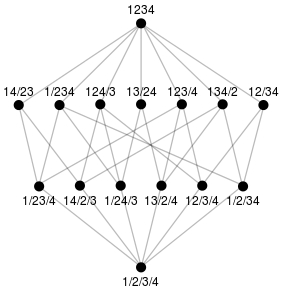
\includegraphics[scale=1]{Reticulo.jpg}   
	\caption{Retículo de subgrupos.}
	\label{Reticulo}
   \end{figure}

  \begin{theorem}[Teorema\IS de Lagrange]
   Si G es un grupo finito y H un subgrupo de G, entonces el número de elementos de H divide el número de elementos de G.
  \end{theorem}
  
  \begin{lemma}
   Sea $\varphi: G\rightarrow G$, son equivalentes:
   \begin{enumerate}
    \item $\varphi$  es inyectiva.
    \item $\varphi$  es biyectiva.
    \item $\varphi$  es sobreyectiva.
   \end{enumerate}
  \end{lemma}
  La demostración de este teorema es totalmente trivial. Con apoyarnos en que el conjunto G es finito, puede observarse que una de
  esas propiedades implica directamente las demas.
  
  \begin{lemma}
   Si $\varphi$  es un biyección y $A, B$ son subconjuntos de $G$:
   \begin{enumerate}
    \item $\text{card}(A)=\text{card}(\varphi(A))$
    \item $A=B \dimplies \varphi(A)=\varphi(B)$
    \item $\varphi(A\cap B)=\varphi(A)\cap\varphi(B)$
   \end{enumerate}
  \end{lemma}
  
  \begin{lemma}
   Sea G un grupo finito y $g \in G$, entonces $\varphi_{g}(x)=g\ast x$. Además, por la propiedad cancelativa, podemos ver que $\varphi_{g}$ es inyectiva.
   
   Además, por ser G finito, sabemos que $\varphi_{g}$ es biyectiva.
  \end{lemma}
  También podemos definir $\varphi_{g} H=\{g\ast h\tq h\in H\}$
  
  \begin{defn}[Clase\IS lateral]
  \[  gH=\varphi_{g}(H) \]
  \end{defn}

  \begin{corol} 
  \label{corol1}
  Extraemos las siguientes conclusiones:
   \begin{enumerate}
    \item $g \in gH$
    \item $\text{card}(H)=\text{card}(gH)$
    \item $H=gH \dimplies g \in H$ 
   \end{enumerate}
  \end{corol}

  \begin{proof}
   \begin{enumerate}
    \item $e \in  H$. Por tanto $g\ast e =g$ que por hipótesis está en $gH$.
    \item Se puede ver apoyándonos en los lemas anteriores puesto que H es finito.
    \item $\Rightarrow$):  $e \in H \implies e=gh$ con $h \in H$. Por lo tanto $h=g^{-1} \in H$ y entonces $g \in H$.\\
	  $\Leftarrow$):  $g \in H \implies g^{-1}\in H$ y todo elemento $h \in H$ cumple $h=g(g^{-1}h)\in H$.
   \end{enumerate}
  \end{proof}
  
  \begin{prop}
   Dados $g_{1}, g_{2}\in G$ y $H<G$, entonces \[ g_{1}H=g_{2}H \] y \[g_{1}H\cap g_{2}H=\emptyset \]
  \end{prop}
  
  \begin{proof}
   La intersección $g_{1}H\cap g_{2}H$ no será vacía si y sólo si $\exists\, h_{1},h_{2} \in H$ tal que $g_{1}h_{1}=g_{2}h_{2}$. Operando 
   \begin{gather*}
   h_{1}=g_{1}^{-1}g_{2}h_{2} \\
   h_{2}^{-1}h_{1}=g_{1}^{-1}g_{2}
   \end{gather*}
   
   Por ser $h_2$ y $h_1$ pertenecientes a $H$, tenemos que $g_{1}^{-1}g_{2} \in H$. Usando la propiedad 3 de (\ref{corol1}), nos queda que
    \[ g_{1}^{-1}g_{2}H=H  \] y por lo tanto \[ g_{2}H=g_{1}H \]
  \end{proof}
  
  \begin{example}
   Tomando el famoso grupo $D_{4}$, podemos obtener H=$\{1,g,g²,g³\}$; sH=$\{s,sg,sg²,sg³\}$
  \end{example}
  
  
  
  \subsection{Particiones}

  \begin{defn}[Relación\IS de equivalencia]
   Fijado un conjunto $G\neq\varnothing$. Una relación $\rel$ en $G$ es de equivalencia si cumple las siguientes propiedades:
  
   \begin{description}   
    \item[Reflexiva] $\forall x\in G \;  x\rel x$
    \item[Simétrica] $\forall x,y \in G\;  x\rel y \dimplies y \rel x$
    \item[Transitiva] $\forall x,y,z \in G\;  x\rel y \y  y\rel z \implies x\rel z$
   \end{description}  
  \end{defn}
 
  \begin{defn}[Partición]
   Familia de subconjuntos disjuntos dos a dos tales que su unión constituye el total. 
  \end{defn}
  
  Una partición define una relación de equivalencia y viceversa. Si $\rel$ es una relación de equivalencia en un grupo $G$, 
  definimos una partición en la que los subconjuntos (clases de equivalencia) son de la forma: \[ S_{x}=\{y\in G \tq x\rel y\} \]
  
  \begin{proof} Definimos una relación de equivalencia $\rel$ en $G$ a partir del grupo $H$:
  
   \[ g_{1}\rel g_{2} \Leftrightarrow g_{1}^{-1}g_{2}\in H \]  y comprobamos que, efectivamente, esta relación es de equivalencia.
   
   Tenemos $S_{e}=H$. Así $S_{g}$  o ya cubre junto con H todo G, o cojo otro $g^{'}$  y repito el proceso con $S_{g^{'}}$.
   Así formare una serie de grupos de la forma $S_{x}$  disjuntos dos a dos y cuya unión me da G.\\
   De esta forma podemos ver que $\card{G}=\card{H}  s$
  \end{proof}
  
  \begin{theorem}[Teorema\IS de Lagrange]
   Dado $g \in  G$, siendo $G$ un grupo finito, entonces $\ord{g}$ divide a $\card{G}$. 
  \end{theorem}
  
  Una interpretación rápida de este teorema es que si el cardinal de $G$ es primo, los únicos subgrupos que tiene $G$ son los triviales: $\gen{e}, G$
  
  \begin{theorem}
   Si el cardinal de $G$ es primo, entonces $G$ es cíclico. Además, si $|G|=n$, entonces \[ \ord{g} | \, n \; \forall g\in G\] y $g^n = e$.
  \end{theorem}
  
  \begin{example}
   Con ayuda de este teorema puede demostrarse el pequeño teorema de Fermat. 
   Definimos $\ent/p\ent=\{\bar{0},\bar{1}...,\bar{p-1}\}$.
   Si tomamos el grupo de las unidades de $\ent/p\ent$ tenemos $\{\bar{1}, \bar{2},....\bar{p-1}\}$ $\Rightarrow$
   $\bar{a}\in\ent/p\ent \wedge \bar{a}\neq 0 \Rightarrow a^{p-1}=\bar{1}$.
  \end{example}
  
  \begin{theorem}
   Si $|G|=p^{2}$  con $p$ primo entonces $\exists g \in G \tq \ord{g}=p$
  \end{theorem}
  
  \begin{proof}
   Tomamos $g\in G \y g\neq e$. Entonces sólo hay dos posibilidades, o bien $\ord{g}=p$ o bien $\ord{g}=p^{2}$. En el primer caso ya lo tenemos, y en el segundo tenemos que existe $g^p$ que tiene orden $p$.
  \end{proof}
  
  \begin{example}
   Por todo lo explicado anteriormente, si tomamos el anillo de polinomios $\ent/p\ent[x]$, tenemos \[ X^{p-1}-\bar{1}=
   \prod_{\bar{a}\in\ent/p\ent \wedge \bar{a}\neq 0}(x-\bar{a}) \]
  \end{example}
  
  \begin{theorem}[Teorema\IS de Lagrange]
   Dados $H<G$,  se cumple que \[ \exists a_{1},\dotsc,a_{r}\in G\tq G=a_{1}H \cup a_{2}H \cup \dotsb \cup a_{r}H\] y que \[ a_{i}H\cap a_{j}H=\emptyset \forall i\neq j\] 
   Es decir, $\card{G}=r\card{H}$
  \end{theorem}

  Definimos ahora otra relación a partir de $H<G$: \[ c\rel^{'}d \Leftrightarrow cd^{-1}\in H \]. La comprobación de que esto es una relación
  la omitiremos por ser trivial. En esta partición, el conjunto de elementos relacionados con d es: $Hd=\{hd\tq h\in H\}$
  
  \begin{defn}[Subgrupo\IS normal]
   Decimos que $H<G$  es un subgrupo normal si \[ gH=Hg \; \forall g \in G \]. Por tanto, si $G$ es un grupo abeliano, $H$ también lo será y cualquier  subgrupo será normal. Un subgrupo normal se expresa como $H\lhd G$.
  \end{defn}
  
  \begin{example}
   Tomamos $G=\ent$  y $H=4\ent$. 
   El subgrupo de los elementos que son equivalentes a n es nH=$\{n+4k\tq k \in \ent\}$.
   En este caso tenemos 4 subgrupos según esta condición: $\bar{0},\bar{1},\bar{2},\bar{3}$
  \end{example}
  
  Si $H\lhd G$  podemos definir una estructura de grupo en el subconjunto de clases, lo que se llamará el grupo cociente.
  
  \begin{defn}[Grupo\IS cociente] Sea $H \lhd G$. Definimos $G / H$ como el conjunto de todas las clases laterales izquierdas, es decir
  
  \[ G/H = \{ aH \tq a \in G\} \]
  \end{defn}
  
  
  Dados $g_{1}H$  y $g_{2}H$  podemos formar el conjunto $\{h_{1}\ast h_{2}\tq h_{1}\in g_{1}H \wedge h_{2}\in g_{2}H\}$. Si operamos   $g_{1}H\ast g_{2}H=(g_{1}\ast g_{2})H$  que es otra clase. Por tanto el grupo de clases es cerrado.
  
  El neutro sería la caja $H$ puesto que $gHH=gH$ para cualquier $g$ que escojamos. Además el inverso de $gH$ es $g^{-1}H$.
  
  Por último, vemos que $(g_{1}H\ast g_{2}H)\ast g_{3}H=g_{1}H\ast Hg_{2}\ast g_{3}H=g_{1}H\ast Hg_{3}\ast g_{2}H$, por ser G asociativo. Queda probado pues, que el conjunto de las clases de equivalencia, forma un grupo.
  
\begin{defn}[Índice\IS de un subgrupo]\label{defIndiceSG} El índice de un subgrupo $H$ de $G$ es el \textit{tamaño relativo} de $H$ en $G$, el número de \textit{copias} de $H$ que llenarían $G$.  

Estrictamente, se define $[G:H]$ es el número de clases laterales de $H$ en $G$. Si $H$ y $G$ son finitos, entonces 

\[ [G:H] = \frac{\card{G}}{\card{H}} \]
\end{defn}
  
  \begin{theorem}
   \[ H< G \y [G:H]=2 \implies H \lhd G \]
  \end{theorem}
  
  \begin{proof}
   Por un lado tenemos que $g\notin H \implies gH= H^{c}$. Por otro lado, si tomamos la otra relación de equivalencia, a partir de $g \notin H obtenemos Hg=H^{c}$.
   
   Uniendo estos dos ejemplos, donde mantenemos H como una mitad en ambos, tenemos Hg=gH. Por tanto H es un subgrupo normal.
   
   Guille: Me lo creo pero me convence cero. ¿Qué es $H^c$? ¿Cuál es la otra relación de equivalencia?
  \end{proof}
  
  \begin{lemma}
   Dadas dos particiones formadas por los subconjuntos $aH$ y $Ha$ para un elemento $a \in G$ y con $H <G$, podemos definir dos aplicaciones $\pi$ y $\pi '$ que lleven cada elemento de G a su respectiva caja \textit{¿qué es una caja?}:
   \[ \appl{\pi}{G}{G/H} \]
   \[ \appl{\pi'}{G}{G/H} \]
   
   Tenemos entonces que:
   
   \[ H \text{subgrupo normal} \implies a_iH = Ha_i \]
   \[ H \text{subgrupo normal} \implies \pi \ =\ \pi ' \]
   
   Además, si H es normal
   \begin{enumerate}
	\item Podemos definir una operación en el conjunto cociente.     
	\item $\appl{\pi}{G}{G/H}$ es compatible con las operaciones.
   \end{enumerate}
  \textit{Pues vale.}
  \end{lemma}
  
\begin{defn}[Centro de un grupo]
	Llamamos centro del grupo $G$ al grupo formado por todos los elementos que conmutan con todos los elementos de $G$.:\\
	\[ Z(G) = \{ a\in G\tq a\ast g = g\ast a\ \forall g\in G\} \]
	Además, tenemos que:
	\[ aZ(G)=Z(G)a \implies Z(G)\lhd G \]
  \end{defn}  
  
  \begin{example}
	Sea $Q$ el grupo formado por las raíces cuartas de 1:
	\[ Q = \{ 1, i, j, k, -1, -i, -j, -k\} \] 
	
	Podemos ver que $Q$ se genera a partir de los elementos $i, j, k$: $Q = \gen{i,j,k}$.
	Además vemos que $-1$ conmuta con todos los elementos del grupo: $-1 \in Z(Q)$
	Analizamos el retículo del grupo y vemos que esta formado por los subgrupos:
	
	\begin{gather*}
	Orden\; 1 = \{ 1\}\\
	Orden\; 2 = \{ 1, -1\} \\
	Orden\; 4 = \{ 1, i, i^2, i^3\},\
			  \{ 1, j, j^2, j^3 \},\
			  \{ 1, k, k^2, k^3 \}.\\
			  \end{gather*}
			  
		  
	El grupo no es abeliano, sin embargo, todos sus subgrupos son normales porque todo subgrupo $H<G$ de índice 2 (es decir, el conjunto de clases $G/H$ tiene dos elementos) es normal.
	
  \end{example}
  
 
 Dados un grupo G y un subconjunto no vacío S, defino $S^{-1}=\{s^{-1}\tq s\in S\}$. Dados $S_{1},S_{2}<G$, defino  \[ (S_{1}\ast S_{2})^{-1}=\{s_{1}\ast s_{2}\tq s_{1}\in S_{1} \wedge s_{2}\in S_{2}\} \]
 
 que operando, nos queda que 
 
 \begin{align*}
 (S_1 \ast S_2)^{-1} &= \{s_{1}^{-1}\ast s_{2}^{-1}\tq s_{1}\in S_{1} \wedge s_{2}\in S_{2}\}\\
 &= \{s_{1}^{-1}\ast s_{2}^{-1}\tq s_{1}^{-1}\in S_{1}^{-1} \wedge s_{2}^{-1}\in S_{2}^{-1}\} \\
 & =S_{2}^{-1}\ast S_{1}^{-1}
 \end{align*}
 
 Sea H un subgrupo de G, entonces $H^{-1}=H$.
 
 \begin{theorem}
  Fijado un grupo G y $H_{1}, H_{2}$  subgrupos de G entonces: $H_{1} \lhd G \implies H_{1}\ast H_{2}<G$. 
 \end{theorem}
 
 \begin{proof}
  Sabemos que $H_{1}\ast H_{2}=H_{2}\ast H_{1}$. Para ver que $H_{1}\ast H_{2}<G$  hay que comprobar que está
  \begin{enumerate}
   \item Cerrado por la operación: $(H_{1}\ast H_{2})\ast (H_{2}\ast H_{1})=H_{1}\ast (H_{2}\ast H_{2})\ast H_{1}=H_{1}\ast H_{1}\ast H_{2}\ast H_{2}=H_{1}\ast H_{2}$
   \item Todo elemento tiene inverso, es decir: $\alpha\in H_{1}\ast H_{2}\Rightarrow \alpha^{-1}\in H_{1}\ast H_{2}$. Pero entonces tenemos:
   $\alpha^{-1}\in (H_{1}\ast H_{2})^{-1} = H_{2}^{-1}\ast H_{1}^{-1}=H_{2}\ast H_{1}=H_{1}\ast H_{2}$ que también contiene a $\alpha$ \textit{por ejemplo.}
  \end{enumerate}

 \end{proof}

 \begin{example}
  Tomamos el ya famoso grupo $D_{4}=\{1,g,g^{2},g^{3}, s, sg, sg^{2}, sg^{3}\}=\gen{s,g}$.
  
  Dentro de este grupo, el elemento 1 tiene orden dos, los elementos $g$, $g^{3}$  tienen orden 4 y el resto, 2.
  \begin{gather*}
  Z(D_{4})= \{\alpha\in D_{4} \tq \alpha\beta=\beta\alpha \ \forall \beta \in D_{4}\}= \\
  = \{\alpha\in D_{4}\tq \alpha s = s\alpha \wedge \alpha g = g\alpha\}=\{1, g^{2}\}=\gen{g^{2}}
  \end{gather*} 
  
  Este subgrupo es normal.
  
  Para contruir el retículo de subgrupos tomamos, en primer lugar, el único grupo de un elemento: 
  \[ \{1\} \]
  Ahora tomamos los grupos de orden dos, que serán todos aquellos generados por elementos que tienen orden dos:\\
  \[ \gen{sg^{3}}, \gen{sg}, \gen{g^{2}}, \gen{s}, \gen{sg^{2}} \]
  
  Los subgrupos de orden cuatro son los formados por elementos de orden 4 más los obtenidos al combinar el centro con los demás subgrupos de orden 2:
  \[ \{1,g,g^{2},g^{3}\}, \ \gen{g}, \ \{1, g^{2}, s, sg^{2}\} \]
 \end{example}
 

 \begin{proof}
 \begin{enumerate}
  \item $\Rightarrow$  Obvio, tan obvio como que $D_4$ le apasiona al profesor.
  \item $\Leftarrow$\\
  $aHa^{-1} \subset H \ \Rightarrow \ a^{-1}Ha\subset H.$. Por tanto $a^{-1}aHa^{-1}a \subset a^{-1}Ha \ \Rightarrow \ a^{-1}Ha \subset  a^{-1}Ha \Rightarrow \ H \subset a^{-1}Ha$.
  Contención a derecha e izquierda implica igualdad.
 \end{enumerate}
 \end{proof} 
 
 \subsection{Homomorfismos de grupos}
 \begin{defn}[Homomorfismo]
 Sea f $\appl{f}{(G_1, \cdot )}{(G_2, \ast )}$. $f$ es un homomorfismo de grupos si 
 \[ f(a\cdot b) = f(a)\ast f(b) \]
 \end{defn}
 
 \begin{example}
 Si consideramos la aplicación $\appl{\pi}{G}{G/N}$ que lleva los elementos de $G$ a su respectivo conjunto cociente, la función sobreyectiva $\pi$ es un homomorfismo de grupos si $N\lhd G$.
 \end{example}
 
 \begin{props} 
 Si $\appl{f}{G_1}{G_2}$ es un homomorfismo de grupos, entonces
 \begin{enumerate}
 \item $f(e_1) = e_2$ con $e_1$ neutro de $G_1$ y $e_2$ neutro de $G_2$
 \item $f(x^{-1}) = f(x)^{-1}$
 \end{enumerate}
 \end{props}
 
 \begin{proof} 
 1) 
 \begin{align*}
 e_1\cdot e_1 &= e_1 \\
 f(e_1)& =f(e_1\cdot e_1) = f(e_1)\ast f(e_1) \\
 f(e_1) &= e_2 \ast e_2 = e_2
 \end{align*}

 2) \begin{align*}
 f(x\cdot x^{-1}) &= f(e_1) = e_2 \\ 
 f(x)\ast f(x^{-1}) &= e_2 \\
  f(x^{-1}) &= f(x)^{-1}
  \end{align*}
 
 \end{proof}
 
 

\begin{remark} Si $G$ es un grupo finito \[\ord{f(a)}\ |\;\ord{a}\, \forall a \in G_1 \] \end{remark}

\begin{lemma}
La composición de dos homomorfismos de grupos es un homomorfismo de grupos.
\end{lemma}

\begin{defn}[Núcleo\IS de un homomorfismo]
Dado $\appl{f}{G_1}{G_2}$ el núcleo de $f$ se define como 

\[ \ncl{f} = \{ a\in G_1 \tq f(a) = e_2\} \]

con $e_2$ el elemento neutro de $G_2$. 

Además, se cumple que $\ncl f = \{ e_1 \}$ si y sólo si $f$ es inyectiva.
\end{defn}

\begin{theorem}
 Sea $\appl{f}{G_1}{G_2}$ un homomorfismo de grupo. Entonces $\ncl f$ y $\img f$ son subgrupos de $G_1$ y $G_2$ respectivamente, con $\ncl f$ el núcleo de la aplicación y $\img f$ la imagen de la misma.
 \end{theorem}
 
 \begin{proof} Empezamos demostrando que el núcleo es un subgrupo.
 \begin{gather*}
  \ncl f < G_1 \\
 e_1 \in \ncl f \\
 x, y \in \ncl f \implies xy^{-1}\in \ncl f \\
 f(xy^{-1}) = \underbrace{f(x)}_{e_2} \underbrace{f(y)^{-1}}_{e_2^{-1}} = e_2
 \end{gather*}
 
Pasamos ahora a demostrarlo con la imagen.

\begin{gather*}
\img f < G_2 \\
 e_2\in \img f \implies e_2 = f(e_1)\\
 a\in \img f \implies a^{-1}\in \img f\\
 \exists \alpha \in G_1 \tq a=f(\alpha ) \implies a^{-1} = (f(\alpha ))^{-1} = f(\alpha ^{-1})
 \end{gather*}
 
 \end{proof}

\begin{defn}[Epimorfismo]
Sea $\appl{f}{G_1}{G_2}$ un homomorfismo de grupos. Entonces diremos que $f$ es un epimorfismo si $\img f = G_2$.
\end{defn}

\begin{defn}[Monomorfismo]
Sea $\appl{f}{G_1}{G_2}$ un homomorfismo de grupos. Entonces diremos que $f$ es un monomorfismo si $\ncl f = \{ e_1\} $
\end{defn}

\begin{lemma} Sea $\appl{f}{G_1}{G_2}$ un homomorfismo de grupos, entonces se tiene que

\[ \ncl f \lhd G_1 \]
\end{lemma}

\begin{proof} Recordemos la definición de subgrupo normal:
\[ H \lhd G_1 \dimplies \forall a\in G_1\ aHa^{-1}\subset H \]
En este caso, tenemos que
\[ \forall a\in G_1\ a\ncl{f}a^{-1} = \{aha^{-1} \tq h\in \ncl{f} \} \]

Si tomamos $f\left(a\ncl{f}\inv{a}\right)$, vemos que es igual a \[ f(a) f(\ncl{f}) f(\inv{a}) = \alpha e_2 \inv{\alpha} = e_2 \]
\end{proof}

\begin{remark}El único homomorfismo de $\ent/n\ent$  en $\ent$, y en general de un grupo finito a los enteros, es el trivial. Esto se debe
a que dado $a\in\ent/n\ent$, ord(a)=$\alpha$, pero $\ord{f(a)}$ será infinito, salvo que $f(a)=0$.\end{remark}
  
\begin{lemma} Si $N\lhd G$ entonces $G/N$ tiene estructura de grupo y $\appl{\pi}{G}{G/N}$  (homomorfismo que manda cada
elemento a su grupo cociente)  es un epimorfismo.
\end{lemma}

\begin{lemma} Dado $\appl{f}{G_1}{G_2}$, con $N=\ncl{F}$ y $N \lhd G$, entonces
\[ b\in aN \dimplies  a^{-1}b\in N \dimplies f(a^{-1}b)=e_2 \ \dimplies f(a)^{-1}f(b)=e_2 \ \dimplies f(a)=f(b) \]
\end{lemma}

\begin{defn}[Isomorfismo]
Un homomorfismo de grupos $\appl{f}{G_1}{G_2}$ es un isoformismo si existe un homomorfismo de grupos $\appl{g}{G_2}{G_1}$ tal que $g\circ f = id_{G_1}$ y $f\circ g = id_{G_2}$. 
\end{defn}

\begin{remark} Dados dos grupos $G_1$ y $G_2$, $\appl{f}{G_1}{G_2}$ es un isomorfismo de grupos si y sólo si f es un homomorfismo y es una biyección de conjuntos.
\end{remark}

\begin{lemma}\label{lemPropsHF}
Sea $\appl{f}{G_1}{G_2}$, entonces:
\begin{enumerate}
\item Si $H_1$ es un subgrupo de $G_1$, $f(H_1)<G_2$
\item Si $H_2 < G_2$, entonces $f^{-1}(H_2)<G_1$
\item Si $H_2 \lhd G_2$, $f^{-1}(H_2)\lhd G_1$
\item Si $f$ es sobreyectiva y $H_1\lhd G_1$, tenemos que $f(H_1)\lhd G_2$
\end{enumerate}
\end{lemma}

\begin{proof}
\paragraph{Propiedad 1}
\begin{gather*}
e_2 \in f(H_1)\\
x, y\in f(H_1) \implies xy^{-1}\in f(H_1)\\
x=f(a);\; y = f(b);\; a, b\in H_1\\
xy^{-1}=f(a)f(b)^{-1} = \underbrace{f(ab^{-1})}_{H_1} \in f(H_1)
\end{gather*}

\paragraph{Propiedad 2}
\begin{gather*}
\\ e_1 \in f^{-1}(H_2)\\
a, b \in f^{-1}(H_2) \implies ab^{-1} \in f^{-1}(H_2)\\
f(a) \in H_2;\; f(b) \in H_2 \implies \underbrace{f(ab^{-1})}_{f(a)f(b)^{-1}}\in H_2
\end{gather*}

\paragraph{Propiedad 3}
$f^{-1}(H_2) = N(\pi \circ f)$. Como $f^{-1}(H_2)$ es el núcleo de h de g entonces $f^{-1}(H_2)\lhd G_1$.
\end{proof}


Sea $\appl{f}{G_1}{G_2}$ un homomorfismo de grupos, y $f$ sobreyectiva (es decir, un \textit{epimorfismo})
vamos a analizar el retículo de subgrupos de $G_2$.\\
Fijado un subgrupo $H_2<G_2$ le asociamos un subgrupo $f(H_2)<G_1$. Asociamos al retículo de subgrupos de $G_2$ subgrupos de $G_1$ que contienen al núcleo $N(f)$.
\begin{theorem}
Es posible identificar el retículo de subgrupos de $G_2$ con los subgrupos de $G_1$ que contienen al núcleo $N(f)$
\end{theorem}

\obs Sea $\appl{f}{G_1}{G_2}$ sobreyectiva. $H$ subgrupo de $G_1$ que contiene al núcleo $N(f)$. Entonces $H = f^{-1}(f(H))$
Como $f(H)$ es un subgrupo de $G_2$ la observación indica que todo subgrupo de $G_1$ que contiene al núcleo es de la forma $f^{-1}(K)$ para algún subgrupo K de $G_2$

\begin{example}
El retículo de subgrupos de $Q/{\{ -1, 1 \} }$ se identifica con los subgrupos de $Q$\footnote{Grupo de cuaterniones, osea, raíces cuartas de uno.} que contienen al núcleo $\{ 1, -1\} $.
\end{example}

\begin{defn}[Grupos\IS isomorfos]
Dos grupos son isomorfos si existe un isomorfismo entre ellos.
\end{defn}

\begin{theorem}\label{thmIsomorfia1}
Si $\appl{f}{G_1}{G_2}$ es un homomorfismo de grupos entonces $Img(f)$ (subgrupo de $G_2$) es isomorfo al grupo cociente $G_1/{N(f)}$\footnote{Recordad que $\ncl f \lhd G_1$}
\end{theorem}

\begin{example}
Si tenemos la aplicación 
\begin{gather*}
\appl{h}{\mathbb{Z}}{\mathbb{C}^*}\\
1 \longrightarrow i\\
k\longrightarrow ik\\
\end{gather*}

$\ncl f = 4\mathbb{Z} < \mathbb{Z}$\\
$Img(f) = \{1, i, -1, -i \}$
Tenemos que $\{ 1, i, -1, -i \}$ es isomorfo al grupo $(\mathbb{Z} /4\mathbb{Z}, +)$
\end{example}

\begin{defn}[Biyección]
 Un homomorfismo $\appl{f}{G_1}{G_2}$ es una biyección si \\
 $\exists \ \appl{h}{G_2}{G_1} \tq \ f\circ h =id \ en \ G_1 \ y\ h \circ g = id \ en \ G_2$.
\end{defn}
Para decidir si un homomorfismo de grupo $\appl{f}{G_1}{G_2}$  es un isomorfismo o no, basta con ver si $f$  es una biyección.\\

Siendo $\appl{f}{G_1}{G_2}$ un isomorfismo se cumple que:
\begin{enumerate}
 \item ord(f(g))=ord(g)
 \item A partir de f se establece una identificación con el retículo de subgrupos
 \item Dos grupos isomorfos comparten propiedades hasta el punto de no poderlos distinguir. (Equivalente a cuando no distinguíamos
 dos espacios vectoriales isomorfos).
\end{enumerate}

\begin{theorem}[Teoría de isomorfismos]
 Siendo N(f)$\lhd$G, con $\appl{f}{G_1}{G_2}$ y $\appl{\pi}{G_1}{G_1/N(f)}$se cumple:
 \begin{enumerate}
  \item $\exists \appl{f^{'}}{G_1}/N(f){G_2} \ \tq f=f^{'}\pi$
  \item $f^{'}$  es un homomorfismo de grupos
  \item $f^{'}$  es inyectiva.
  \item Img(f)=Img($f^{'}$)
 \end{enumerate}
\end{theorem}
\begin{proof}
 \begin{enumerate}
  \item Si tomamos $f^{'}(\bar{a})=f(a)$  tenemos que ver que está bien definido, es decir, que no depende del representante escogido.\\
  $\bar{a^{'}}=\bar{a} \Leftrightarrow a^{'}N(f)=aN(f) \ \Leftrightarrow a^{'}\in N(f)a \ \Leftrightarrow \ f(a^{'})=f(a)$
  \item Probamos ahora que es un homomorfismo de grupos:\\
  $ f^{'}(\bar{a}\bar{b})=f^{'}(\bar{ab})=f(ab)=f(a)f(b)$
  \item Veamos ahora la inyectividad\\
  $\bar{a}\in N(f) \Leftrightarrow f^{'}(\bar{a})=e_2 \ \Leftrightarrow \ f(a)=e_2 \ \Leftrightarrow \ a\in N(f) \ \Leftrightarrow \ \bar{e}=bar{a}$
  \item Se cumple por ser $\appl{\pi}{G_1}{G_1/N(f)}$.
 \end{enumerate}
\end{proof}

\begin{theorem}[Teorema 1 de isomorfía]
 Si $\appl{f}{G_1}{G_2}$  es un isomorfismo de grupos sobreyectivo, entonces $G_2$  es isomorfo al grupo $G_1/N(f)$.
\end{theorem}
\begin{proof}
 Sabemos que $f^{'}$  es un homomorfismo inyectivo y como $\pi$  es sobreyectivo Img(f)=Img($f^{'}$)=$G_2 \ \Rightarrow f^{'}$ sobreyectiva.\\
 Por tanto, $f^{'}$  es una biyección.
\end{proof}
\begin{corol}
 Si G es cíclico de orden n, entonces G es isomorfo a ($\mathbb{Z}/n\mathbb{Z}$, +)
\end{corol}

\begin{notacion}
$G_1 \simeq G_2$ es decir que $G_1$ isomoforfo a $G_2$.
\end{notacion}

\begin{example}
Si tenemos un grupo $G$ cíclico, tal que el orden de $G$ es $n$ entonces sabemos que
$\exists a \in G \tq ord(a) = |G|$
Si tomamos el homomorfismo siguiente:\\
$$\appl{f}{\mathbb{Z}}{G}$$\\
$$k \longrightarrow a^k$$\\
es sobreyectiva y su núcleo son los multiplos de $n$ ($n\mathbb{Z}$)
El primer teorema de isomorfía dice que $G \simeq \mathbb{Z}/\ncl f  = \mathbb{Z}/n\mathbb{Z}$
\end{example}

Otra manera de ver el teorema de isomorfía es el siguiente.
\begin{theorem}[Teorema 1 de isomorfía (II)]
Sea $\appl{f}{G}{G'}$ un homomorfismo de grupos, entonces $Img(f) \simeq G/\ncl{f}$
\end{theorem}

\begin{lemma}
 Dado un homomorfismo de grupos $\appl{f}{G}{G'}$  con N(f)$\vartriangleleft$G.\\
 Sea $N_1 \vartriangleleft N(f) \vartriangleleft G$. Entonces existe $\bar{f}$, homomorfismo de grupos tal que $\bar{f}\circ\pi=f$.\\
 Se tiene ademas que Im($\bar{f}$)= Im(f) por ser $\pi$  sobreyectiva.
\end{lemma}
\begin{proof}
 La demostración de este lemma es idéntica a la de la teoría de isomorfismos. Sólo hay que cambiar N(f) por $N_1$.
\end{proof}

Vamos a ver ahora cuantos homomorfismos existen de la forma $\appl{f}{\mathbb{Z}}{G}$. Siendo G infinito\\
En general, existen tantos homomofismos como elementos tenga el grupo G. Para ver esto, vamos a construirlos.\\
Si al 1 le asociamos un elemento $a \in$G, a cada elemento k le asociamos $a^{k}\in$G. Por tanto, tenemos homomorfismos como valores
podamos asociar al 1 y tenemos tantos valores posibles como elementos de G.\\
\\
Ahora vemos que pasa si tomamos $\appl{f}{\mathbb{Z}/n\mathbb{Z}}{G}$. \\
En este caso el homomorfismo queda determinado por f($\bar{1}$) porque
f($\bar{2}$)=f($\bar{1}+\bar{1}$)=f($\bar{1}$)f($\bar{1}$). Además ord(f($\bar{1}$)/ord($\bar{1}$)=n\\
El lema anterior nos permite ver que el recíproco de esta afirmación es cierto.\\
\begin{proof}
Construyo $\appl{f}{\mathbb{Z}}{G}$  con g(1)=$a\in G$ con N(g)=n$\mathbb{Z}$  y n=ord(a)
Puedo aplicar el lema anterior $\Rightarrow \exists \appl{f}{\mathbb{Z}/n\mathbb{Z}}{G} \ \tq f(1)=a$. (Esta sería la $\bar{f}$ del lema).
\end{proof}

Por tanto, para ver cuántos homomorfismos hay de la forma $\appl{f}{\mathbb{Z}/n\mathbb{Z}}{A}$, tengo que ver cuántos elementos
de A tienen un orden que divida a n (para mandar allí el $\bar{1}$)\\

\begin{lemma}
 Dados $N\vartriangleleft N' \vartriangleleft G$, puedo dividir G en "cajas" a partir de la relación de equivalencia basada en N. Es decir,
cada "caja" tendrá los elementos de la forma g$N$  con g$\in G$. Por otro lado, puedo hacer este mismo proceso con $N'$.\\
Se observa pues, que las cajas de $N'$  esta formada por la unión de cajas de $N$. Por tanto tenemos que $N'/N \vartriangleleft G/N$.\\
\end{lemma}

\begin{theorem}[Teorema 2 de isomorfía]
 Dados $N_1\vartriangleleft N_2 \vartriangleleft G$  se tiene que:
 \[ (G/N_1)/(N_2/N_1)\backsimeq G/N_2\]
 Donde $\backsimeq$  denota isomorfo.
\end{theorem}

\begin{proof}
 Como $N\vartriangleleft G  \wedge  N_1 \lhd N_2$, aplicando el lema 1.58 tenemos que existe un epimorfismo $\appl{\bar{\pi}}{G/N_1}{G/N_2}$.\\
 Aplicando el teorema 1 de isomorfía tenemos que $G/N_2 \backsimeq (G/N_1)/N(\bar{\pi})$. Si logramos probar que el núcleo de $\bar{\pi}$ 
 es lo mismo que $N_2/N_1$  ya estará finlizada la demostración.\\
 El núcleo de la aplicación $\bar{\pi}$  son aquellos elementos de $G/N_1$  que van a $\bar{e}$, es decir, aquellos elementos que pertenecen a $N_2$.
 Si una clase de tipo $\bar{g}\in N_2 \Rightarrow g \in N_2$. Por tanto el núcleo está formado por aquellas clases de equivalencia de elementos pertenecientes a $N_2$.
 Es decir, el núcleo es $N_2/N_1$. (Si no lo ves claro piensa que las clases de elementos de G se representaban como $G/N_1$, ahora es lo mismo pero
 no son elementos de G sino de $N_2$  porque quiero el núcleo.).
\end{proof}

\begin{example}
 Vamos a ver un ejemplo de como construir homomorfismos.\\
 Supongamos que quiero construir un homomorfismo $\appl{f}{D_3}{G}$.\\
 Por lo explicado anteriormente, este homomorfismo quedará determinada por la imagen de los generadores de $D_3$. Por tanto,
 basta con escoger dos elementos de $G$  y asignarlos $f(s)=\alpha, \ f(g)=\beta$  de tal forma que: ord($\alpha$)/ord($f(s)$) y ord($\beta$)/ord($f(g)$).\\
 Pero además, estos dos elementos deben cumplir la última propiedad que me definía $D_3$: $f(s)f(g)=(f(g))^{-1}f(s)$
\end{example}

\begin{defn}
Dados H, K dos subgrupos de G, siendo H un subgrupo normal, HK es el menor subgrupo de G que contiene a ambos.
\end{defn}

 Si tenemos $H \vartriangleleft G \ \appl{\pi}{G}{G/H}$, dado un $\bar{K} < G/H, \  H \subset \ \pi^{-1}(\bar{K}) < G $, por ser $e_2 < \bar{K}$. Por otro lado, todo subgrupo de G que contiene a H cumple que $K=\bar{\pi}^{-1}(\bar{\pi}(K))=$.
 
 \begin{example}
  Dados $H=d_1\mathbb{Z}, \ , K=d_2\mathbb{Z}$, HK es el menor subgrupo que los contiene, por tanto $HK=d\mathbb{Z}$, con d=m.c.d.($d_1, d_2$).
 \end{example}

 \begin{theorem}
  Todo subgrupo de $\mathbb{Z}/n\mathbb{Z}$  es cíclico de la forma <$\bar{d}$>, donde d divide a n y ord(<$\bar{d}$>)=n/d.
 \end{theorem}
\begin{example}
 Tenemos $\bar{K}\in \mathbb{Z}/n\mathbb{Z}$  con subgrupos <$\bar{d_1}$>, <$\bar{d_2}$>,..., <$\bar{d_r}$> con r divisor de n.\\
 Si ahora genero <$\bar{K}$> quiero ver con que subgrupo coincide.\\
 Tomo $\appl{\pi}{\mathbb{Z}}{n\mathbb{Z}}$.\\
 Sabemos que $n\mathbb{Z}=N(\pi) \subset \pi^{-1}(\bar{K})$  y también sabemos que $\bar{K} \in \pi^{-1}(\bar{K}$. Es decir,
 la contraimagen debe contener a k y a n. Por tanto debe contener a k$\mathbb{Z}$  y a n$\mathbb{K}$, por lo que es el subgrupo
 d$\mathbb{Z}$  con d=m.c.d.(k,n).\\
 $\pi(\pi^{-1}(\bar{K}))=\pi(d\mathbb{Z})=<\bar{d}>$, que tiene orden n/d.
\end{example}

Si G es un gurpo cíclico de orden n, entonces es isomorfo a $\mathbb{Z}/n\mathbb{Z} \Rightarrow$  todo subgrupo de G es cíclico y 
tiene tantos subgrupos como divisores positivos tiene n.

\begin{theorem}
 $a\in G \wedge ord(a)=n \ \Rightarrow ord(a^{k})=\frac{ord(a)}{d}$, con d=m.c.d.(n,k)
\end{theorem}

\begin{proof}
 Construyo un homomorfismo $\appl{f}{\mathbb{Z}}{G}$  tal que f(1)=a. \\
 Así tenemos que $<a>\simeq \mathbb{Z}/n\mathbb{Z} \ n=ord(a)$.\\
 Este isomorfismo me lleva $a^{h}\textrightarrow \bar{k}$  y ord($a^{k}$)= ord($\bar{k}$) y  aplicando el teorema anterior tenemos
 que ord($\bar{k}$)=n/d con d=m.c.d.(n,k).
\end{proof}

\begin{defn}[Automorfismo]\label{defAutomorfismo}
 Isomorfismo que nos lleva un conjunto en sí mismo. Aut(G) es el conjunto de automorfismos de G.
\end{defn}

\begin{example}
 Vamos a buscar Aut($\mathbb{Z}$)\\
 g(1)=1 y g(1)=-1 son todos los automorfismos posibles.\\
 Así tenemos Aut($\mathbb{Z}$)=$\{1,-1\}$=$\{f, f^{-1}\}$. Ambas son expresiones del conjunto de automorfismos de $\mathbb{Z}$. Ambas
 consituyen grupos pero con distintas operaciones asociadas. Estas operaciones son la suma y la composición respectivamente.
\end{example}

\begin{example}
 Vamos a buscar Aut($\mathbb{Z}/n\mathbb{Z}$)\\
 Como ya hemos visto, para encontrar homomorfismos de $\mathbb{Z}/n\mathbb{Z}$  basta con definir f($\bar{1}$) = g con ord(g)/n=ord($\bar{1}$).\\
 Estos homomorfismos serán isomorfismos si  ord($\bar{g}$)=n, lo cual ocurre si $\bar{g}\in U(\mathbb{Z}/n\mathbb{Z}) \ \Leftrightarrow g \ coprimo \ con\ n$\\
 Como la composición de isomorfismos es otro isomorfismo, vuelve a cumplirse que Aut($\mathbb{Z}/n\mathbb{Z}$)  es un grupo.
\end{example}

Para que una aplicación de un conjunto finito en sí mismo sea una biyección, basta con ver que cumple la propiedad inyectiva o sobreyectiva
ya que las siguientes son consecuencia directa. Es decir, por ser finito, si la aplicación es inyectiva, no le queda otra que ser
también sobreyectiva y por tanto, biyectiva.\\

Sea $\{1,...n\}$=$S_1\coprod S_2\equiv$ unión disjunta y sea $\alpha$  una biyección que fija los elementos de $S_1$  y $\beta$
otra que fija los elementos de $S_2$. En tal caso, estas biyecciones conmutan.\\
En general, si $\alpha$,  $\beta$  son biyecciones disjuntas se cumple que:
\begin{enumerate}
 \item $\alpha \circ \beta = \beta \circ \alpha$
 \item $\alpha^{k}, \beta^{l}$  son también biyecciones disjuntas, ya que siguen dejando fijos los elementos de `$S_1$  y $S_2$  respectivamente.
\end{enumerate}

\begin{defn}[Ciclo]
Fijado ($i_1, i_2,...,i_r$)$\subset$(1,2,3,...n), un ciclo es una biyección que lleva cada elemento $i_i$  al siguiente $i_{i+1}$, y deja
fijos los demás elementos de (1,2,3,...n).
\end{defn}

\begin{theorem}
 Toda biyección puede expresarse de forma única como la composición de biyecciones disjuntas
\end{theorem}
\begin{proof}
 Dada una aplicación, reconozco sus ciclos y la combinación de ellos me dará la aplicación. En realidad estoy reescribiendo los
 cambios que realiza la aplicación en forma de ciclo y dejando los elementos que la aplicación dejaba quietos igual. \\
 Por ser los ciclos biyecciones disjuntas, el efecto de uno no interfiere en otro.\\
\end{proof}
Veamos esto más claro con un ejemplo.
\begin{example}
 Tenemos la aplicación $\sigma$=(2,3,1,4,6,5,7,9,8,10). Vamos a buscar sus ciclos. Para ello, cojo un elemento y voy viendo donde
 lo mandan sucesivas aplicaciones de la función hasta volver a mi punto de partida.\\
 Empezamos con el 1. Aplicando sucesivamente la aplicación, observo las siguientes transformaciones: 1$\Rightarrow$2$\Rightarrow$3$\Rightarrow$1. Ya
 tenemos un ciclo. Este ciclo será representado como (1,2,3) según la notación indicada en la definición de estos ciclos.\\
 Ahora tomo otro elemento que no esté incluido ya en este ciclo. 4 $\Rightarrow$4. Este sería un ciclo con un único elemento, sería
 la identidad, que no es necesario representar.\\
 Tomo ahora 5 $\Rightarrow$ 6 $\Rightarrow$ 5. Tenemos aquí un ciclo de orden dos (5,6)\\
 Tomo ahora 7 y veo que estamos en el mismo caso que el 4.\\
 Tomo el 8 $\Rightarrow$ 9$\Rightarrow$8. Tenemos otro ciclo de orden dos (8,9).\\
 El 10 nos queda invariante.\\
 Por tanto tenemos que nuestra aplicación $\sigma$ = (1,2,3)(5,6)(8,9). Es decir, si a un conjunto de 10 elementos ordenados le aplico
 estos tres ciclos, obtengo el mismo resultado que aplicándole directamente la aplicación $\sigma$.
\end{example}

Ahora vamos a demostrarlo.

\begin{proof}
Fijamos un $\sigma \in S_n$. Sea $X = \{ 1,2,\hdots ,n\} $.\\
Vamos a crear una partición definiendo la siguiente relacion:\\
$a,b \in X$, $aRb$ si $\sigma ^i(a) = b$ para algun $i\in \mathbb{N}$\\

Lo primero que vamos a hacer es comprobar que la relación define una partición.
\begin{enumerate}
\item $\forall a \in X$, $aRa$, $\sigma ^{n!} (a) = a$.
\item $aRb \implies bRa$ es decir:\\
 $\exists i \tq \sigma ^i (a) = b \implies \exists j \tq \sigma ^j = \sigma ^{-i}$\\
 $\sigma ^j (b) = a$.
\item $aRb$ y $bRc$ $\implies aRc$. Para verlo partimos de que:\\
 $\exists i \tq \sigma ^i (a) = b $\\
 $\exists j \tq \sigma ^j (b) = c $\\
 Tenemos pues $c=\sigma^j(b)=\sigma^j(\sigma ^i(a))=\sigma^{i+j}(a)$


\end{enumerate}

Por tanto sabemos que la relación define una partición.
Si tomamos el grupo $C(a) = \{ a, \sigma (a), \hdots , \sigma ^N(a), \hdots \} $\\
Si $\sigma ^s (a)=a \implies |C(a)| \leq S$.\\
Sea $r$ el menor entero positivo tal que $\sigma^r(a)=a$\\
Concluimos que card$(\{ a, \sigma (a), \hdots , \sigma ^{r-1}(a)\}) = r =$ card(C(a))\\
Así que $\sigma = \sigma _1 \circ \hdots \circ \sigma _s$
donde $\sigma _i = \{ a, \sigma (a), \hdots , \sigma ^r(a)\} $ con $r$ la longitud del ciclo.
\end{proof}

\begin{defn}[Trasposición]
$(ab)$ un ciclo de longitud 2 es una trasposición.
Es decir, que fija elementos en $\{ 1,2, \hdots , n\} \{ a, b\} $\\
$a\longrightarrow b$\\
$b\longrightarrow a$\\
\end{defn}

\begin{theorem}
Todo $\sigma \in S_n$ se obtiene como composición de trasposiciones.
\end{theorem}

\begin{example}
Sea $\sigma$ un ciclo de longitud r. \\
$\sigma = ( a, \sigma (a), \sigma ^2(a), \hdots, \sigma ^{r-1}(a)) =
(a, \sigma ^{r-1}(a))\ast \hdots (a, \sigma ^2(a)) \ast(a, \sigma (a) $
\\Ambas funciones son iguales porque toman los mismos valores en el conjunto \\ $\{a, \sigma (a),\hdots , \sigma ^{r-1} (a) \}$ y ambas fijan a los elementos en $X / \{a, \sigma (a),\hdots , \sigma ^{r-1} (a) \}$ 
\end{example}

\obs Como toda permutación es composición de ciclos y todo ciclo es composición de transposiciones, resalta que toda permutación es composición de transposición. Obvio, que diría \href{http://www.uam.es/personal_pdi/ciencias/dyakubov/dimitry.jpg}{\color{blue}{Dmitry}}.

% % % % % % % % % % % % % % % % % % % % % % % % % % % % % % %

\subsection{Automorfismos interiores de un grupo}

Fijado un elemento $g\in G$ definimos $\appl{\phi _g}{G}{G}$ de forma que la imagen
de un punto $a$ de $G$ sea $\phi _g(a) = gag^{-1}$.

Se puede ver que $\phi$ es una biyección y un homomorfismo de grupos, es decir, es un isomorfismo de grupos. Demostrémoslo comprobando que $\phi_g(ab) = \phi_g(a)\phi_g(b)$. 

Tenemos que
\begin{gather*}
\phi _g (a) = g a g^{-1}\\
\phi _g (b) = g b g^{-1}\\
\end{gather*}

Operando, vemos que
\[ \phi _g (a b) = g (a b) g^{-1} = g (a g^{-1} g b) g^{-1}) = (ga\inv{g}) (g b \inv{g}) = \phi _g (a) \phi _g(b) \]

Es por lo tanto un homomorfismo de grupos, y al ser biyección es un isomorfismo de grupos: está claro que $\phi _{g^{-1}} \phi _g = \phi _g \phi _{g^{-1}} = id_G$

Con esto, tenemos que, fijado un elemento $g\in G$, podemos definir un isomorfismo $\appl{\phi _g}{G}{G}$. Podemos definir entonces una aplicación que lleve cada elemento a su automorfismo correspondiente:  

\begin{defn}[Interior\IS de un grupo] Definimos el interior de un grupo como el conjunto de sus automorfismos generados de la forma que acabamos de exponer:
\begin{align*}
 \appl{In&}{G}{Aut(G)} \\
 In(g) &= \phi_g
 \end{align*}
 
 De tal forma que el conjunto imagen se define como
 
\[ In(G) = \{ \phi_g \tq g\in G\} \subset Aut(G) \]

donde $Aut(G)$ es el conjunto de automorfismos (\ref{defAutomorfismo}) de $G$.
\end{defn}

Es fácil de ver que si $G$ es abeliano, cualquier aplicación $\phi_g$ será la identidad ($\phi_g(a) = g a \inv{g} = g\inv{g}a = a$) y por lo tanto $In(G) = \{ id_G \}$.

\begin{theorem}
Fijado un grupo G, se tiene que
\begin{itemize}
\item $In(G) < Aut(G)$
\item $In(G)$ es isomorfo a $G/Z(G)$
\end{itemize}
\end{theorem}

\begin{proof}
Primero, demostramos que la función $appl{In}{G}{Aut(G)}$ que lleva cada $g$ en $\phi _g$ es un homomorfismo de grupos y $N(In) = Z(G)$. Es decir, hay que comprobar que $\phi_g\circ \phi_{g'} = \phi_{gg'}$:

\[ \phi _g \circ \phi _{g'} (a) = g(g'a\inv{g'})\inv{g} == (gg')a(gg')^{-1} = \phi_{gg'} (a) \]
 
 Una vez que sabemos que $In$ es un homomorfismo, podemos aplicar sus propiedades (ver lema \ref{lemPropsHF}), por las que tenemos que
 
 \[ \img(G) < Aut(G) \]

y además, según el primer teorema de isomorfía (\ref{thmIsomorfia1}) 

\[ \img(In) = G/N(In) \]
\end{proof}

\begin{example}
En el caso $G = S_n$\footnote{Aquel grupo de las permutaciones de elementos}
tenemos que si la aplicación $\appl{\phi}{G}{G}$ es un isomorfismo, entonces $ord(a) = ord(\phi (a))$ porque $ord(\phi (a)) | ord(a)$ y $ord(a) | ord(\phi (a))$.\\
Si $\sigma$ es el ciclo de longitud $r$\\
$\sigma(a_1, a_2, \hdots, a_r)$ donde \\
$a_1 \longrightarrow a_2$\\
$a_2 \longrightarrow a_3$\\
$\hdots$\\
$a_r \longrightarrow a_1$\\

Entonces vemos que $\phi (\sigma) = (g(a_1), g(a_2), \hdots, g(a_r)) = grg^{-1}$
es decir, que la imagen de $\sigma$ por $\phi _g$ es un ciclo de longitud $r$.\\

Hay que probar esto viendo si:
$(g\sigma g^{-1})(g(a_1)) = g(a_2)$\\
$(g\sigma g^{-1})(g(a_2)) = g(a_3)$\\
$\hdots$\\
$(g\sigma g^{-1})(g(a_r)) = g(a_1)$\\
\\
probamos el primero viendo que: \\
$(g\sigma g^{-1})(g(a_1)) = g\sigma(a_1) = g(a_2)$
el resto se prueban igual.
\end{example}

\subsubsection{Particiones definidas por el interior de un grupo}

 Podemos ver que el homomorfismo $\appl{In}{G}{Aut(G)}$ define una partición en X, o lo que es lo mismo, define una relación de equivalencia:
 
 \[ a\rel b \iff \exists g \in G \tq φ{g}(a)=b ]\]


Es decir, que dos elementos $a,b \in G$ están relacionados si hay una biyección $\varphi_{g}$  que los relaciona. Demostremos que, efectivamente, $\rel$ es una relación de equivalencia.

\begin{proof}
 \paragraph{Propiedad reflexiva} $\forall a, aRa$
 
 Está claro que esta propiedad se cumple: tomamos la biyección $φ_{e}$, donde $e$ es el elemento neutro, y tenemos que 
 
 \[ φ_e(a)=a \implies a\rel a\]
 
 \paragraph{Propiedad simétrica} $\forall a,b, a\rel b\implies b\rel a$
 
 Operando con dos elementos $a,b$
    \[ gag^{-1}=b \implies a=g^{-1}bg \]
    
 Es decir, \[ \varphi_{g}(a)=b\Rightarrow \ \varphi_{g^{-1}}(b)=a \]
 
 y por lo tanto se cumple la propiedad simétrica.
 
 \paragraph{Propiedad transitiva} $a\rel b \wedge b\rel c \Rightarrow \ a\rel c$
 
 	Partimos de que
    
    \[ gag^{-1}=b \ \wedge \ g_{2}bg_{2}^{-1}=c\]
    
    Sustituyendo $b$ tenemos que 
    \[ gg_{2}ag_{2}^{-1}g^{-1}=c\ \Rightarrow \varphi_{gg_{2}}(a)=c \]

\end{proof}

Vamos a estudiar ahora el caso en el que $G=S_{n}$. Queremos conocer que "pinta" tiene cada caja en este caso. Recordemos que 
$S_{n}$  es el grupo de biyecciones de un conjunto sobre sí mismo (en este caso el conjunto sería X).\\
Veamos un ejemplo concreto
\begin{example}
 Sea $S_{4}$  vamos a hallar los equivalentes a $\sigma$=(1,2,4). Estos equivalentes son de la forma $g\sigma g^{-1} \tq g \in S_{4}$.\\
 Dado que $S_{4}$  consta de 24 elementos, es inmanejable la idea de escribirlos todos. Además, incrementando n, el número de elementos
 aumentaría de forma increible.\\
 Dado $g\in S_{4}$  se cumple que $g(1,2,4)g^{-1}=(g(1),g(2),g(4))$.\\
 Para comprobarlo basta con ver que $g(1,2,4)g^{-1}(g(1))=g(2)$  y repetir esta observación con los demás elementos del ciclo.\\
 Por tanto, generalizando esta idea, vemos que en la caja de (1,2,4) estará cualquier treciclo. Por tanto, cada caja obtenida tendrá
 ciclos de 1,2,3 ó 4 elementos.\\
 Como cualquier biyección puede expresarse de forma única como composición de ciclos disjuntos se tenemos:\\
 $\varphi_{g}(\sigma)=g\sigma g^{-1}\ = \ \varphi_{g}(r_{1}) \circ \varphi_{g}(r_{2}) \circ ... \circ \varphi_{g}(r_{s})$. Donde $r_{i}$  son cada uno de los
 ciclos que componen la biyección.\\
 Se cumple que $\varphi_{g}(\sigma)=g(r_{1})g^{-1} \circ ... g(r_{n})g^{-1}$.  Por tanto en la misma caja están aquellas biyecciones que se descomponen
 en el mismo número de ciclos disjuntos con los mismos tamaños de cada ciclo.
\end{example}

\begin{defn}[Clase\IS de equivalencia]
Fijado un elemento $a\in G$, definimos la clase de equivalencia o clase conjugada $cl(a) \subset G$ como el subconjunto de la partición de $G$ que contiene al elemento $a$. Más formalmente:

\[ cl(a) = \{ b \in G \tq b\rel a \} = \{ gag^{-1} \tq g \in G \} \]
\end{defn}

\begin{remark} De la definición de clase de equivalencia podemos Si $a = e$ es el elemento neutro, entonces $cl(e) = \{ geg^{-1} \tq g\in G\} = \{ e\} $ y por tanto $\card{cl(e)} = 1$. 

También se puede ver que si $G$ es un grupo abeliano $cl(a) = \{ gag^{-1} \tq g \in G\} = \{ a \}$.
\end{remark}

\begin{example}
Si tomamos el grupo de las permutaciones $G=S_4$ y lo expresamos como composición de ciclos disjuuntos, tenemos:\\
\begin{center}
\begin{tabular}{|l|r|}
\hline
& Tipo\\ 
\hline
(1) & 1\\
(1 2) & 2\\
(1 2)(3 4) & (2 2)\\
(1 2 3) & 3\\
(1 2 3 4 & 4\\
\hline
\end{tabular}
\end{center}
Si $G=S_4$\\
$$\appl{In}{S_4}{Aut(S_4}$$
tenemos que, por tomar un par de casos
$cl((1\ 2)) = \{ \text{Permutaciones de tipo 2} \}$\\
$cl((1\ 2)(3\ 4)) = \{ \text{Permutaciones de tipo 2, 2]} \}$\\
y así podemos definir\\
$S_4 = cl((1)) \coprod cl((1\ 2)) \coprod cl((1\ 2)(3\ 4)) \coprod cl((1\ 2\ 3)) \coprod cl((1\ 2\ 3\ 4))$
\end{example}

Está claro que $In$ define una relación de equivalencia en $G$. Si tomamos $\card{G/\rel} = s$, y $\{x_n\}∈G$ representantes de las clases de equivalencia, tenemos trivialmente que 

\[ \card{G} = \sum_{i=1}^{s} \card{cl(x_i)} \]

Pero en esa definición tenemos un problema: ¿Cuánto vale $\card cl(a)$?

Para responder a esa pregunta, empecemos definiendo lo siguiente:

\begin{defn}[Centralizador] Dado $\appl{In}{G}{Aut(G)}$ y un elemento $a$ de $G$, definimos el centralizador $C$

\[ C(a) = \{ g\in G \tq \phi _g(a) = a\} = \{ g\in G \tq gag^{-1} = a\} \]

Este es el conjunto de elementos que no mueven al elemento a por $\phi$
\end{defn}

\begin{theorem}\label{thmConj1}
Fijado $a\in G$, tenemos que
\begin{enumerate}
\item $C(a) < G$
\item $[ G:C(a) ] = \# cl(a) $ 
\end{enumerate}
\end{theorem}

Esto es, se mira el índice (\ref{defIndiceSG}) en $G$ de los elementos que no mueven a $a$ para ver cuántos elementos tiene la clase de $a$.

\begin{proof}
\paragraph{1)} Recordamos la definición del centralizador: $C(a) = \{ g\in G \tq \phi _g(a) = a\} = \{ g\in G \tq gag^{-1} = a\}$

Para demostrar que $C(a)$ es un subgrupo de $G$, nos basta con ver que $\forall g_1,g_2∈ C(a)\; g_1g_2 ∈C(a)$. Es trivial ver que si $g_1, g_2 \in C(a)$ la composición $\phi_{g_1}\circ φ_{g_2}$ también lo estará: $\phi _{g_1, g_2}(a) = a$. 

\paragraph{2)} Si $G$ es un grupo finito, los elementos de la clase conjugada de $a$ se corresponden uno a uno con las clases laterales del centralizador $C(a)$. Recordemos la definición de clase lateral: $gH = \{ gh\tq h∈ H\}$. Podemos tomar dos elementos, $b$ y $c$, de tal forma que $b = c z$ con $z∈ C(a)$ y por lo tanto pertenezcan a la misma clase lateral. 

Si calculamos el conjugado vemos que tanto $b$ como $c$ dan como resultado el mismo elemento:

\[ ba\inv{b} = (cz)a\inv{(cz)} = cz a\inv{z} \inv c = cz\inv z a \inv c = c a \inv c \]

Por lo tanto, habrá tantos elementos en la clase de equivalencia como clases laterales distintas tenga $C(a)$. Es decir 

\[ [G:C(a) = \card{cl(a)} \]
\end{proof}

Recordemos el lema que nos muestra que si la clase de equivalencia de un elemento $a$ sólo contiene a un elemento, ese elemento es el $a$ y además $a$ pertenece al centro del grupo $G$, es decir, conmuta con todos los elementos del grupo, sea cual sea el elemento.

\begin{lemma}
Son equivalentes:
\begin{enumerate}
\item $\#cl(a) = 1$
\item $cl(a) = \{ a\}$
\item $a \in Z(G)$
\end{enumerate}
\end{lemma}

\begin{proof}
$cl(a) = \{ a \} \iff gag^{-1} = a \iff ga = ag \iff a \in Z(G)$
\end{proof}

La cuestión es "contar" los elementos que hay en un grupo. Vemos entonces la \textbf{ecuación de clases de conjugados}.


\begin{defn}[Ecuación\IS de clases de conjugados]\label{defEqConj} Sean $\{ x_1, \hdots, x_s \}$ elementos de $G$, elegidos de tal forma que cada $x_i$ pertenece a una clase con al menos 2 elementos. Entonces:

\[  |G| = |Z(G)| + |cl(x_1)| + \hdots + |cl(x_s)| \]

O, lo que es lo mismo,
\[ |G| = |Z(G)| + \sum_{i=1}^{s}[G:C(x_i)] \]
\end{defn}

\begin{defn}[p-Grupo] Dado un número primo $p$, un p-grupo $G$ es un grupo periódico en el que el orden de cada elemento es una potencia de $p$. Dicho de otra forma, por cada $g∈G$, existe un entero $n$ de tal forma que $g^{p^n} = e$.

Un grupo finito es un p-grupo si y sólo si el número de elementos es una potencia de $p$, es decir, que

\[ |G| = p^s\;s∈ℤ \]
\end{defn}

Por ejemplo, se ve fácilmente que $D_4$ es un 2-grupo porque $|D_4| = 8 = 2^3$.

Los p-grupos tienen ciertas propiedades. La primera es que su centro no es el trivial:

\begin{theorem}
Todo p-grupo $G$ finito tiene un centro no trivial
\end{theorem}

\begin{proof} Para la demostración del teorema usaremos la ecuación de clases de conjugados (\ref{defEqConj}): 

\[  |G| = |Z(G)| + \sum_{i=1}^{s}|cl(x_i)| \]

Por (\ref{thmConj1}) sabemos que el orden de una clase de equivalencia de $G$ tiene que dividir al orden de $G$. Como $|G| = p^n$ para algún $n∈Z$, tenemos que el orden de una clase de equivalencia $|cl(g_i)| = p^{k_i}$, con $0<k_1<n$. De esta forma, 

\[ |G|= p^n = |Z(G)| + \sum{i=1}^s p^{k_i} \]

de lo que se sigue que $p$ tiene que dividir en ambos lados de la ecuación y por lo tanto $|Z(G)| > 1$.
\end{proof}

\begin{theorem}
Todo grupo de orden $p^2$ es abeliano. Además, $|Z(G)| = |G|$
\end{theorem}

\begin{proof}
La hacéis vosotros porque \href{http://www.uam.es/personal_pdi/ciencias/villa/imagenes/Foto18.jpg}{\color{blue}{Orlando}} la ha borrado tras escribirla.
La idea es que si el índice de $Z(G)$ fuera igual que $p$, el grupo cociente $G/Z$ es cíclico de orden $p$, y por tanto G sería abeliano. Luego el índice de Z no puede ser $p$ si $G$ no es abeliano y por tanto sería al menos $p^2$. Así que todo grupo de orden $p^2$ no abeliano tendría como centro sólo al elemento neutro y esto es imposible. Por tanto $Z(G)$ es abeliano.
\end{proof}

Los grupos abelianos nos resultan muy cómodos porque tienen la interesante propiedad de que cualquier subgrupo es normal. Por tanto
G/H tendría estructura de grupo para cualquier subgrupo H de G. Además, se puede establecer un isomorfismo entre G y G/H, lo cual también 
resulta muy interesante. Esto nos permite emplear argumentos inductivos en el cardinal de G.\\
Como ejemplo de esta inducción, vamos a volver a demostrar el teorema de Cauchy.
\begin{theorem}[Teorema\IS de Cauchy]
 Si $p$ es primo y divide a $|G|$, entonces $G$ tiene un elemento de orden $p$.
\end{theorem}
\begin{proof}
 Caso base de la inducción:\\
 |G|=1 $\Rightarrow$ G=$\{e\}$ \\
 |G|=2 $\Rightarrow$  G=$<g>$  con ord(g)=2.
 
 Lo que hago ahora es "dividir" por H. Con ello paso a un grupo abeliano de menor orden sobre el que seguir aplicando la inducción.\\
 Supongamos que el teorema se cumple $\forall m < n$  (Hióptesis de inducción).\\
 Sea h$\in G \tq h\neq e\Rightarrow ord(h)=qn' \wedge \ ord(h)| |G|$  con q primo.\\
 Se cumple que $h^{n'}$  tiene orden q. Si q=p, ya está terminada la demostración.\\
 Si p $\neq$ q tomo G'=G/H con H=$<h^{n'}>$  que tendrá orden |G'|=|G|/q.\\
 Observemos que p divide a |G'|. Por inducción aplicamos el teorema en G' que tiene orden menor que n.\\
 Por tanto $\exists \bar{g}\in G' \ \tq ord(\bar{g})=p$.\\
\end{proof}

\begin{defn}[Inducción]
 En estos ejercicios la inducción consiste en:
 \begin{enumerate}
  \item Probar el caso base
  \item Considerar que el teorema a demostrar es válido para cualquier n menor que el que yo tengo
  \item Demostrar que lo que quiero demostrar equivale a demostrarlo con otro grupo con menor cardinal. Este grupo suele obtenerse
  de la forma G/H con H $\vartriangleleft$ G. De esta forma se da G/H $\backsimeq$ G y tiene sentido la inducción.
 \end{enumerate}
\end{defn}


\begin{theorem}[Teorema\IS de Sylow (1)]
 Sea p primo, $|G|=p^{r}m$  con $p, r$ coprimos. Entonces $G$ tiene un subrupo de orden $p^{r}$.\\
 Es decir, $|G|=p^{a}q^{b} \ \Rightarrow$  existen subgrupos de orden $p^{a}$  y $q^{b}$
\end{theorem}
\begin{proof}
 Vamos a demostrarlo por inducción.\\
 |G|=$p^{r}m \Rightarrow \ \exists H < G \ \tq \ |H|=p^{r} \ \Rightarrow$  H contiene un elemento de orden p\\
 
 Para aplicar la inducción consideramos el caso base probado por ser trivial. Y consideramos que el teorema es válido para cualquier cardinal
 menor que n.
 \begin{itemize}
  \item Caso 1: p | card(Z(G))\\
    Existirá un ismorofismo que irá de G a G/H con H < Z(G) y nos encontramos en la misma situación que cuando G era abeliano.\\
    Por tanto, aplicando el teorema de Cauchy, tenemos que existe un elemento en Z(G) con orden p y en concreto existe H < Z(G) con |H|=p.\\
    Tomo ahora $\appl{\pi}{G}{G/H}$. Tenemos que |G/H|=$p^{r-1}m$. Por inducción sabemos que G/H tiene un grupo con cardinal $p^{r-1}$  al que
    llamaremos $\bar{N}$.\\
    Sabemos que existe $\pi^{-1}(\bar{N}) < G$  y que $\pi^{-1}(\bar{N}) /H=\bar{N}$.\\
    Como |H|=p y suponemos que |$\bar{N}$|=$p^{r-1}$  tenemos que $\pi^{-1}(\bar{N})$  tiene $p^{r}$  elementos.
    
  \item Caso 2: p $\nmid$  card(Z(G))\\
  Para la demostración de este caso, será útil recordar la ecuación de clases.\\
  Si tengo G finito, tomo $\appl{Inn}{G}{Aut(G)}$  que define una partición del conjunto G en subconjuntos de la forma cl(a)=$\{gag^{-1} \tq g\in G\}$
  Asociamos a cada elemento a $\in$ G un subgrupo de elementos que fijan a, C(a). Ya probamos que [G:C(a)]=$\#$cl(a).\\
  $\#cl(a)=1 \Leftrightarrow \forall g\in G \ gag^{-1}=a \ \Leftrightarrow \forall g \in G \ ga=ag \ \Leftrightarrow a \in Z(G)$.\\
  La ecuación de clases nos decía que:
  Sean $\{ x_1, \hdots, x_s \}$ elementos de $G$, cada $x_i$ pertenece a una clase con al menos 2 elementos. Entonces: \\
  $$|G| = |Z(G)| + |cl(x_1)| + \hdots + |cl(x_s)|$$
  $$|G| = |Z(G)| + \sum_{i=1}^{s}[G:C(x_i)]$$
  
  Si tomo ahora el módulo p tenemos que |$\bar{G}$|=$\bar{0}$. Por hipótesis sabemos que $\bar{|Z(G)|} \neq 0$. Por tanto, dentro del 
  sumatorio debe haber algún elemento distinto de 0 módulo p. Tomo este elemento $[G:C(X_i)]$  y formulo la ecuación ya
  demostrada:\\
  \[|G|=[G:C(X_i)]|C(X_i)|=p^{r}m\] Este cardinal es divisible por p. 
  Sabemos que, tal y como lo hemos escogido, $[G:C(X_i)]$  no es divisible por p. Por tanto tiene que darse $|C(X_i)|=p^{r}m'$  con m y p coprimos.\\
  Puesto que $C(X_i) \varsubsetneq G$  tiene cardinal menor que n y por lo tanto podemos aplicar de nuevo inducción.
 \end{itemize}

\end{proof}

Vamos a resolver algunos ejercicios de la hoja 4 para poner en práctica lo estudiado hasta la fecha.
\begin{itemize}
 \item Ejercicios 7, 8 y 9\\
 Dado $\sigma \in S_n$, el signo de $\sigma$  será 1 si es producto de un número par de trasposiciones o -1 si es producto de un número
 impar de estas.\\
 Sea $\sigma = t_1...t_r=p_1...p_s$  con $t_i, p_j$  trasposiciones. Entonces $p_1..p_s t_1...t_r=1$.\\
 r+s es par, por lo que r y s tienen la misma paridad.
 
 Tomamos $\appl{sg}{S_n}{\{1,-1\}}$  que es un homomorfismo de grupos.\\
 Dados $\sigma=t_1...t_r,  \sigma'=t_1^{'}...t_r^{'}$, sg($\sigma \sigma'$)=$(-1)^{r+r'}$, porque sg($\sigma$)=$(-1)^r$  y sg($\sigma'$)=$(-1)^{r'}$.\\
 Ker(sg)=$A_n \equiv$Subgrupo alternado. Es el subgrupo de elementos de signo 1. Al ser un núcleo es un subgrupo normal.\\
 $S_n/A_n\simeq \{\pm 1\} \ \Rightarrow |S_n/A_n|=2=|S_n|/|A_n| \ \Rightarrow \ |A_n|=n!/2$\\
 
 \item Ejercicio 10\\
 Tomamos $S_3$=$\{1, (123), (132), (23), (13), (12)\}$\\
 $(123)=(12)(23), (132)=(13)(32)$\\
 $A_3=\{1, (123), (132)\} \simeq C_3$
 
 \item Ejercicio 11\\
 Recordamos que el temorema de Lagrange me dice que dado un grupo finito G se cumple:
 \[H<G \Rightarrow |H| \ divide\ |G|\]
 Dado |$A_4$|=4!/2=12. Queremos ver que no tiene ningun subrupo de cardinal 6.\\
 
 a) Vamos a ver que $A_4$  tiene 8 elementos de orden 3.\\
 $\sigma\in A_n \wedge ord(\sigma)=3 \ \Rightarrow \ \sigma$  es un 3-ciclo.\\
 Como cada permutación puede expresarse de forma única como composición de trasposiciones, vamos a ver de cuantas formas podemos 
 descomponer 4. Por ejemplo tenemos 4=3+1=2+2=2+1+1=1+1+1+1.\\
 Los tipos de elementos en $S_4$  son, según la descomposición que hemos hecho del 4, de la siguiente forma:\\
 (abcd),(acb),(ab)(cd),(ab), 1 contando a,b,c,d distintos.\\
 
 Los órdenes de estos elementos son, respectivamente, 4,3,2,2,1. Todos ellos tienen signo 1 salvo (ab) y (abcd) que tienen signo -1.\\
 Para ver el orden simplemente descomponemos la biyección en trasposiciones y vemos si tenemos un número par de ellas.\\
 El número de 3-ciclos en $S_4(\circ A_4))$(Un 3-ciclo siempre está en $A_4$, por tanto contando los 3-ciclos de $S_4$  estoy 
 contando a la vez los de $A_4$) es 4*2=8. Donde 2 es el número de 3-ciclos  en $S_3$  y 4 el número de soportes posibles (nº subconjuntos
 de 3 elementos).\\
 
 b)Dado H<$A_4$, con |H|=6 tomamos a $\in A_4$  con ord(a)=3.\\
 Vamos a comparar $a, \ aH, \ a^{2}H \in A_4/H$. \\
 Por lo que sabemos de los grupos cocientes, estos elementos son disjuntos o iguales.\\
 Recordemos que $xH=yH \Leftrightarrow \ y^{-1}x\in H$.  Por tanto\\
 $H=aH \Leftrightarrow a\in H$\\
 $aH=a^{2}H \Leftrightarrow a\in H$\\
 $H=a^{2}H \Leftrightarrow a^{2}\in H \ \Leftrightarrow a \in H$\\
 
 ¿Pueden ser disjuntos estos grupos? \\Difícilmente por que cada uno de ellos tiene 6 elementos. Si fuesen disjuntos tendríamos ya localizados
 18 elementos de $A_4$, que hemos dicho que sólo tiene 12 elementos. Por tanto sólo nos queda la opción de que estos tres grupos 
 sean iguales y a $\in$ H.\\
 Sin embargo, en este caso a$\in$ H es cualquier elemento de orden tres de $A_4$.\\
 $\{a \tq a \in A_4, ord(a)=3\}\subset H$\\
 $|\{a \tq a \in A_4, ord(a)=3\}|$=8>6 ERROR.\\
 Lo que falla es la existencia del grupo H.
 
 \item Ejercicio 12\\
 Vamos a probar que la relación $aRb \Leftrightarrow \exists f\in Inn(G) \tq f(a)=b$, es una relación de equivalencia:
 \begin{enumerate}
  \item $aRa \Leftrightarrow 1a1^{-1}$
  \item $aRb \Leftrightarrow \exists x \tq xax^{-1}=b \Leftrightarrow a=x^{-1}bx\Leftrightarrow bRa$
  \item $aRb \wedge bRc \Leftrightarrow \exists x,y \tq xax^{-1}=b \wedge yby^{-1}=c \Leftrightarrow yxax^{-1}y=zax^{-1}c \Leftrightarrow aRc$
 \end{enumerate}
 Ahora definimos la clase de equivalencia de a según esta relación:\\
 cl(a)=$\{xax^{-1} \tq x \in G\} = \{f(a) \tq f \in Inn(G)\}$
 
 \item Ejercicio 13\\
 Si el conjunto es abeliano, la clase de equivalencia de un elemento está formada por ese único elemento debido a que si G es abeliano,
 $\forall x \in G \ xax^{-1}=xx^{-1}a=a$.\
 
 \item Ejercicio 14\\
 Recordemos que dos elementos conjugados tienen el mismo orden.
 \begin{proof}
  $aRb \Leftrightarrow \exists f \in Inn(G) \tq f(a)=b$  f es un automorfismo de G y conserva órdenes.
 \end{proof}
 Aplicando esto, vemos que las clases de este grupo son: $\{1\}$, $\{a, a^{2}\}$, $\{a^{2}, ab, a^{2}b\}$\\
 Esto puede deducirse porque:\\
 $bab^{-1}=a^{-1}=a^{2}$\\
 $aba^{-1}=a^{2}ba^{-2}=a^{-1}ba=a^{-2}b=ab$\\
 Estas ecuaciones se infieren de las condiciones que definen $D_3$ de forma abstracta: $ab=a^{1}b$\\
 
 \item Ejercicio 15\\
 Recordamos que en $S_4$  los tipos de elementos (tipos de estructuras de ciclos) eran (abcd),(acb),(ab)(cd),(ab), 1\\
 Los conjuntos de elementos de $S_4$  que tienen uno de estos tipos (prefijado) son clases de conjugación\\
 \begin{proof}
  Tomamos por ejemplo cl((abcd))= $\sigma (abcd) \sigma'= \tau$\\
  $\tau(\sigma(1))=\sigma(2)$  y sucesivamente. Así obtenemos
  $\tau = (\sigma(1)\sigma(2)\sigma(3)\sigma(4))$
 \end{proof}

 Este cálculo podría repetirse con cualquier ciclo. Ya lo vimos en la teoría pero siempre viene bien repetir, al fin y al cabo, de eso trata esta asignatura.
\end{itemize}

Sea $X$ un conjunto finito cualquiera, construimos el grupo formado por las biyecciones de $X$ en $X$ y la operación composición: $Biy(X) = \{\appl{f}{X}{X}\ \text{biyección}\}$. Ahora vamos a definir una relación de equivalencia en el conjunto $X$ definiendo así una partición utilizando un homomorfismo de grupos: $\appl{l}{G}{Biy(X)}$.\\

La relación de equivalencia que vamos a definir es la siguiente:\\
$a$ y $b$ están relacionados si existe una biyección que lleve el $a$ en $b$:\\ $aRb \iff \exists g\in G \tq \phi _g(a)=b$\\

Veamos que esto define una relación de equivalencia:\\
\begin{enumerate}
\item $\forall a \in X\ aRa$\\Para demostrar esto tomamos la identidad.
\item $a,b \in X\ aRb \implies bRa$\\$\exists g \ \phi_g(a) = b \implies \exists g' \tq \phi _{g'}(b) = a$\\Para demostrar esto tomamos la función inversa.
\item $aRb \wedge bRc \implies aRc$\\$(\exists g_1\in G \tq \phi_{g_1}(a) = b) \wedge (\exists g_2\in G \tq \phi_{g_2}(b) = c) \implies \exists g_3 \tq \phi_{g_3}(a) = c$\\Para demostrar esto vemos que $g_3$ es la composición de $g_1$ y $g_2$ por ser homomorfismo de grupos.
\end{enumerate}

\begin{defn}[Órbita]
$Si a\in X$ entonces el conjunto de la partición que contiene al elemento $a$ es:\\

$$orb(a) = \{ b\in X\tq aRb\} = \{ \phi_g(a) \tq g\in G\}$$

Es una forma general de llamar a una clase.
\end{defn}

Se plantea el problema de calcular el cardinal de la órbita.
Antes de eso vemos lo siguiente:

\begin{defn}[Estabilizador]
$Stab(a) = \{ g\in G \tq \phi_g (a) = a\} \subset G$
\end{defn}

Y demostramos lo siguiente:
\begin{enumerate}
\item $Stab(a) < G$
\item $[G: Stab(a)] = \# orb(a)$
\end{enumerate}

\obs Dado $G\longrightarrow Biy(X)$, si $X$ es unión de $r$ subconjuntos y si $\{ x_1, \hdots, x_n\} $ son representantes de estos $r$ subconjuntos de la partición:\\
$$|X| = \sum \# orb(x_i) = \sum_{i=1}^r[G:Stab(x_i)]$$

Veamos una aplicación de lo anterior:

\begin{example}
Sea $G$ un grupo y $X = \{ H\tq H<G\} $
Tomamos $G = S_3$ y $X$ es el conjunto de los subgrupos de $S_3$

$X = \{ \{1 \}, \{1, (1,2) \}, \{1, (1,3) \}, \{1, (2,3) \}, <(123)>, S_3 \}$

Definimos un morfismo de $G$ en las biyecciones de $X$: $G\longrightarrow Biy(X)$

Dados $g\in G$ tenemos que $\appl{\phi_g}{G}{G}$ lleva $a$ en $gag^{-1}$\\
$\phi _g$ es un isomorfismo de $G$ en $G$ y define una biyección en $X$.\\
Si $H<G$ entonces $\phi _g(H) = gHg^{-1}$ es un subgrupo de G. Como $\phi_g$ es un isomorfismo, $\phi _g$ establece una biyección entre los subgrupos de $G$.

Como $\phi _g$ es un isomorfismo, tenemos que un subgrupo $H$ y el correspondiente subgrupo de $G=S_3$: $\phi _g(H) = gHg^{-1}$ tienen la misma cantidad de elementos.

Vemos entonces que $S_3 \longrightarrow Biy(X)$ define una partición del conjunto $X$.
Por tanto, dos elementos de $X$ (i.e. $H_1$ y $H_2$ subgrupos de $G$) son equivalentes $\iff H_2 = \sigma H_1 \sigma^{-1}$ para $\sigma \in S_3$

Vamos a anotar un par de observaciones:\\
\begin{itemize}
\item La clase de $\{ 1\}$ es $\{ 1\}$
\item $\{ 1, (1,2)\}$ y $<(1,2,3)>$ no pueden estar en la misma clase porque no existe una biyección de uno a otro por tener diferente número de elementos.
\item Como $<(1,2,3)>$ es el unico subgrupo con 3 elementos, entonces ese subgrupo conforma una clase.
\item $S_3$ conforma otra clase, por el mismo razonamiento que el caso anterior.
\item Los subgrupos de orden 2 están todos en la misma clase.
\end{itemize}

El primer teorema de Sylow dice que el número de elementos de $S_3$ es $6=2*3$, y por tanto hay subgrupos de orden 2 y de orden 3.

El segundo teorema de Sylow (que veremos más adelante) dice que todos los sugrupos del mismo orden están en la misma clase.
\end{example}

Dado un grupo G fijo y un elemento $g\in G$  ya hemos definido el isomorfismo $\appl{\varphi_g}{G}{G}$  y teníamos $\varphi_{g}^{-1}=\varphi_{g^{-1}}$\\
Si fijo un subgrupo H < G entonces $\varphi_g(H)=H'$, isomorfo a H\\
\begin{defn}[Conjugado]
 Decimos que dos grupos A, B son conjugados si $\exists g \in G \tq gAg^{-1}=B$\\
 Por definición, dos grupos conjugados son isomorfos
\end{defn}

Definimos un conjunto X cuyos elementos son los subgrupos de G. El isomorfismo $\varphi_{g}$  manda subgrupos de G en subgrupos de G. 
Es por tanto una biyección de X en X.\\
Debemos tener en cuenta que $H \vartriangleleft G \Rightarrow gHg^{-1}=H \forall g$

\begin{theorem}[1º Teorema de Sylow]
 $|G|=n=p^{\alpha}m$  con p y m coprimos $\Rightarrow \ \exists H < G \tq |H|=p^{\alpha}$. \\
 Decimos que H es un p-subgrupo de Sylow
\end{theorem}

\begin{theorem}[2º Teorema de Sylow]
 $H, H'$  son p-subgrupos de Sylow $\Rightarrow \ gHg^{-1}=H'$
\end{theorem}

\begin{example}
 Tomamos G=$S_3$. $|S_3|$=3!=6=2*3\\
 Tenemos que X=$\{id, <(12)>, <(13)>,<(23)>,<(123)>\}$\\
 Por el primer teorema de Sylow hay un subgrupo de orden 2 (<(12)>) y de orden 3 (<(123>)).\\
 Estas dos afirmaciones se deducen del primer teorema de Sylow porque puedo interpretar una vez que p=2 y m=3 y luego puedo reaplicar
 el teorema considerando p=3 y m=2.\\
 El segundo teorema de Sylow dice que, por ejemplo <(12)>, <(23)> son conjugados\\
 \[g(12)g^{-1}=(g(1)g(2))=(23)\]
 El g que me da esto es el que me garantiza eso es (123).\\
 Vemos además que <(123)> es normal porque no tengo con quien conjugarlo.
\end{example}

\begin{example}
 Tomamos G=$S_4$. $|S_4|$=4!=$2^3*3$\\
 Por el primer teorema de Sylow tenemos: $\exists H < S_4 \tq |H|=8$\\
 Para ver esto por nosotros mismo y corroborar que lo que nos dice el teorema es correcto, vamos a ver la analogía con $D_4$.\\
 El grupo $D_4$  no es bastante conocido y sabemos que tiene 8 elementos. Si asociamos cada vértice del cuadrado con un número distinto
 del 1 al 4, cada movimiento rígido que pertenecía a $D_4$  podemos definirlo como una biyección de $S_4$  viendo qué movimientos hace
 con los vértices. \\
 Por ejemplo, g=(1234) suponiendo que hayamos numerado los vértices en orden, porque me lleva del vértice 1 al 2, luego al 3 y sucesivamente.\\
 Por tanto cada elemento de $D_4$  se corresponde con una biyección de $S_4$. Así el subgrupo formado por las biyecciones (1234) y (14)(23)
 (correspondientes al giro y la simetría) constituye un grupo isomorfo a $D_4$  y por tanto, con orden 8.
\end{example}

\begin{example}
 Si tuviéramos G=$D_4$. $|D_4|$=8=$2^3$.\\
 En este caso el teorema de Sylow no dice nada útil, ya que sólo me garantiza que existe un subgrupo con tantos elementos como el 
 grupo total.
\end{example}

Si tomamos un grupo $G$ y denotamos el conjunto de todos los subgrupos como $X$ tenemos que los subgrupos $H_1, H_2 \in X$ definen una relación de equivalencia $H_1RH_2 \iff H_1 = gH_2g^{-1} \ \forall g\in G$

Recordamos entonces, que $orb(H) = \{ H' \text{equivalente con }H \} = gHg^{-1}\ \forall g \in G$

Asociamos a un subgrupo $H$ de $G$ su normalizador:
$N(H) = \{ g\in G \tq gHg^{-1} = H \}$

Con todo esto vemos que $N(H)<G$ y $H\subset N(H)$. Si $G$ es finito, $N(H)$ es cerrado por la operación.

La cuestión que nos podemos plantear es: ¿por qué este subgrupo se llama normalizador?
\obs $H \lhd N(H)$, que quiere decir que $nH = Hn \ \forall n \in N(H) \iff H = nHn^{-1}\ \forall n \in N(H) \iff orb(H) = \{ H \}$

Fijados $G$ y $X$ tenemos:
\begin{itemize}
\item $orb(H) = \{gHg^{-1} \tq g\in G \} \subset X$
\item $N(H) = \{ g \in G \tq gHg^{-1} = H \}$
\item Y por tanto $\# orb(H) = [G:N(H)]$
\end{itemize}

\begin{example}
$G = S_4$, 
$H = <(1\ 2)>$\\
La órbita de $H$ es $orb(H) = \{ \text{los subgrupos de }S_4 \text{ generados por un } 2-ciclo \}$ que tiene $\#orb(H) = {4 \choose 2} = \frac{4!}{2!2!} = 6$ elementos.

Calculamos el normalizador:\\
Vemos que $[S_4:N(H)] = 6$, y $|S_4|=4!=24$, entonces como $[S_4:N(H)]|N(H)|=|S_4|=4!=24$ el tamaño del normalizador ha de ser $\frac{24}{6}=4$.\\
$H\subset N(H) = \{(1),\ (1\ 2),\ (3\ 4),\ (1\ 2)(3\ 4) \}$

\end{example}

\begin{theorem}[Teorema de Sylow \IS Tercero]
$|G| = n = p^{\alpha} m$, $(m:p) = 1$.\\
Sea $n_p$ el número total de p-subgrupos de Sylow.
$n_p \text{ divide a } m \text{ y }  n_p \equiv 1(mod p)$
\end{theorem}

\begin{example}[Clave de las claves para este examen]
 Tomamos $A_4<S_4$, siendo $A_4$  el grupo de las permutaciones pares de $S_4$, que son la mitad. Por tanto $|A_4|=12=2^{2}3$\\
 Por el primer teorema de Sylow, existen $H_4, H_3$  subgrupos de $A_4$  tales que $|H_4|=4 \ \wedge |H_3|=3$\\
 Por el segundo teorema de Sylow, si $H_2, H_2^{'}$  son subgrupos de orden 4 $\Rightarrow \ H_2^{'}=gH_2g^{-1}$  para algún $g\in A_4$\\
 Por el segundo teorema de Sylow, si $H_3, H_3^{'}$  son subgrupos de orden 3 $\Rightarrow \ H_3^{'}=gH_3g^{-1}$  para algún $g\in A_4$\\
 Por el tercer teorema de Sylow, si $n_2=\#\{2-subgrupos \ de \ Sylow \} \Rightarrow \ n_2|3 \ \wedge n_2\equiv 1 mod(2)$\\
 Por el tercer teorema de Sylow, si $n_3=\#\{3-subgrupos \ de \ Sylow \} \Rightarrow \ n_3|4 \ \wedge n_3\equiv 1 mod(3)$\\
 Atendiendo a lo que indican estos teoremas, $n_2$  podría tomar los valores 1 ó 3\\
 Del mismo modo $n_3$  podría tomar los valores 1 ó 4\\
 Ahora tenemos que ver con cual nos quedamos.\\
 Los 2-ciclos de $S_4$  no están en $A_4$  por ser combinaciones de un único elemento\\
 Los 3-ciclos de $S_4$  si que están en $A_4$\\
 Los 4-ciclos de $S_4$  no están en $A_4$  por ser combinaciones de un número impar de elementos\\
 La identidad también pertenece a $A_4$\\
 Las biyecciones que son combinaciones de dos ciclos disjuntos también están en $A_4$.\\
 En definitiva, $A_4=\{(1), (ab)(cd), (abc)\}$. Del tipo (ab)(cd) tenemos 3 posibilidades (tres formas de elegir a y b, ya que c y d
 están condicionados a esa elección). Del tipo (abc) tenemos 4 posibilidades (4 posible elementos a dejar fuera del 3-ciclo). Así tenemos un
 total de 12 elementos, como indicamos al inicio del ejemplo.\\
 
 El subgrupo de orden 4 que precide el segundo teorema de Sylow no puede contener un 3-ciclo ya que estos tienen orden 3 que no divide
 a 4.\\
 Por fuerza tiene que ser H=$\{(12)(34), (13)(24), (14)(23), (1)\}$. Como $|H|=4=2^{2} \Rightarrow$  es abeliano.\\
 El segundo teorema no dice "nada" en este caso por que sólo hay un subgrupo de orden 4. En este caso H es normal por ser su propio
 conjugado.\\
 Se deduce pues $n_2=1$\\
 
 El subgrupo de orden 3 que precide el teorema no puede contener ningún elemento de la forma (ab)(cd) ya que estos elementos tienen
 orden 2, que no divide a 3. Un subgrupo podría ser, por ejemplo, $H=\{(123),(132),(1)\}$.\\
 Tenemos 4 grupos como este (los obtenemos mirando "a pelo", por lo que $n_3=4$.\\
 \end{example}

 \begin{example}
  Tomamos G con |G|=3*11\\
  Por el primer teorema de Sylow, existen dos subgrupos con 3 y 11 elementos respectivamente\\
  Por el segundo teorema de Sylow, si existen dos grupos con 3 elementos, son conjugados (resp. con 11 elementos)\\
  Por el tercer teorema de Sylow, $n_3=\#\{3-subgrupso \ de \ Sylow\} \Rightarrow n_3|11 \ \wedge \ n_3\equiv 1 mod(3) \ \Rightarrow n_3=1$.
  Sólo hay un subgrupo de orden 3. Por tanto este subgrupo será normal.
 \end{example}

 \begin{lemma}
  Dados $H_3, \ H_{11}$  subgrupos normales de G tales que $H_3\cap H_{11} = \{e\} \Rightarrow \ H_3H_{11} \simeq H_3 x H_{11}$.\\
  Si $|H_3xH_{11}|=|G| \Rightarrow G\simeq H_3xH_{11}$
 \end{lemma}
 \begin{proof}
  Tenemos que $H_1H_2=\{h_1h_2\tq h_1\in H_1 \wedge h2\in H_2\}$\\
  Si probamos que $h_1h_2=h_1^{'}h_2^{'} \Leftrightarrow h_1=h_1^{'} \wedge h_2=h_2^{'}$  entonces queda claro que tenemos tantos elementos como
  $|H_1||H_2|$ (cada elemento de $H_1$  lo combino con los posibles elementos de $H_2$)\\
  Tenemos pues $h_1h_2=h_1^{'}h_2^{'} \Leftrightarrow H_1\ni h_1^{'}h_1=h_2h_2^{'} \in H_2 \Rightarrow h_1^{'}h_1=h_2h_2^{'}=e$  porque son 
  disjuntos los H. Por tanto tenemos que $h_1=h_1^{'} \wedge h_2=h_2^{'}$
 \end{proof}

 Para el teorema anterior basta con que uno de los H fuese normal.\\
 Dado que $H_1, H_2$ son normales, tenemos que dados $h_1\in H_1$  y $h_2\in H_2 \Rightarrow h_1h_2=h_2h_1 \Rightarrow h_1h_2h_1^{'}=e$\\
 Que puede considerarse como el producto de dos elementos de $H_2$  o de $H_1$.\\
 Por tanto podemos definir el homomorfismo $\appl{f}{H_1xH_2}{H_1H_2}$. La condición necesaria y suficiente para que sea un homomorfismo
 de grupos es que $\forall a \in H_1, b \in H_2 \ ab=ba$\\
 Si consideramos el homomorfismo $\appl{\varphi}{H_1\times H_2}{G}$, tenemos que:\\
 $Img(\varphi)=H_1H_2\equiv H_1 \times H_2$. Esto se puede observar apoyándonos en el primer teorema de isomorfía y viendo que el 
 núcleo de esta aplicación es el neutro, es decir, se trata de un monomorfismo.\\
 \[(h_1,h_2=\in N(\varphi) \Leftrightarrow h_1h_2=e \ \Leftrightarrow h_1=h_2^{-1}\in H_1 \wedge \in H_2\]
 Pero el único elemento común de estos grupos es el neutro.\\
 
 \begin{example}
  Queremos ver que todo grupo de orden $7^{2}11$  es abeliano.\\
  Por el primer teorema de Sylow tenemos: \\
  \[\exists H_1, H_2 <G \tq |H_1|=7^{2} \wedge |H_2|=11\]
  Por el tercer teorema de Sylow tenemos que existe sólo un grupo de la forma $H_1$  y un único grupo de la forma $H_2$, por tanto,
  ambos subgrupos son normales.\\
  Vemos que $H_1 \bigcap H_2 = \{e\}$, ya que el elemento que pertenezca a la intersección debe pertenecer a ambos y cumplir $g^49=g^11=e$  
  y esto sólo lo cumple el elemento neutro.\\
  Por tanto, por el lema anterior $H_1\times H_2 \equiv H_1H_2 < G$. Dado que $|H_1H_2|=|G| \Rightarrow H_1H_2=G \Rightarrow G \equiv H_1 \times H_2$
  Por ser $H_1, H_2$  abelianos, tenemos que G es abeliano por ser isomorfo.
  \end{example}

  \begin{example}
   Demostrar que todo grupo de orden 15 es isomoforfo morforforforforfo{\large forforforforforforfo{\LARGE forforforforforforfo{\huge forforforforforforfo {\Huge forforforforforforfo}}}} % JAJAJAJAJAJAJJAAJA ISOMOFORFO SE HA EQUIVOCADO AL ESCRIBIRLO JAJAJAJAJAJA
   a $\mathbb{Z}/n\mathbb{Z}$.\\
   Notemos que si demostramos que todo grupo de orden 15 es cíclico, esto implicará la isomorfía buscada.\\
   Aplicando los teoremas de Sylow, tenemos que existe un único grupo de orden 5 y un único grupo de orden 3. Tal y como vimos en el 
   ejemplo anterior, tenemos que $G\equiv H_1\times H_2$.\\
   Tomemos $(h_1, h_2)\in H_1 \times H_2 \Rightarrow orden((h_1, h_2))=1,3\ o \ 5$.\\
   Sabemos que este orden no es 1 porque consideramos  $(h_1, h_2)\neq (e_1, e_2)$\\
   Vemos que $(h_1, h_2)^{3}=((h_1^{3}, e_2) \ \wedge (h_1, h_2)^{5}=(e_1, (h_2)^{5})$\\
   Por tanto el orden de este elemento no es 3 ni 5, por tanto sólo queda la posibilidad de que sea 15. Por tanto es un grupo cíclico.
  \end{example}

  Vamos a hacer un breve repaso de las principales propiedades de los grupos finitos abelianos.\\
  Sea G un grupo de este tipo, se tiene que:\\
  \begin{enumerate}
   \item Todo subgrupo H de G es normal
   \item Dados $H_1$,  $H_2$, subgrupos de G $\Rightarrow$  $H_1H_2$  es un subgrupo
   \item Dados $H_1$,  $H_2$, subgrupos de G $\Rightarrow$ $\appl{\varphi}{H_1\times H_2}{G}$, siendo $\varphi(h_1,h_2)=h_1h_2$
   \item Para cada p solo existe un p-subgrupo de Sylow
   \item $\forall r \tq r / |G| \ se \ tiene \ que \ G_r\{g \in G \tq g^{r}=e\}$  es un subgrupo
   \item |$G_{p^{\alpha}}$|=$p^{n}$, ya que $G_{p^{\alpha}}$  contiene todos los elementos cuyo orden es una potencia de p.
   \item Por el primer teorema de Sylow podemos garantizar la existencia de este grupo $G_{p^{\alpha}}$
   \item Dados $n_1, n_2 \tq n=n_1n_2=|G| \ \Rightarrow G \equiv G_{n_1}\times G_{n_2}$
   \begin{proof}
    Dado $g \in G$, se tiene que $g^{n}=e$\\
    Sabemos que existen s y t tales que $sn_1+tn_2=1 \ \Rightarrow g=g^{sn_1}g^{tn_2}$\\
    Pero $(g^{sn_1})^{tn_2}=g^{sn_1n_2}=g^{ns}=e \Rightarrow g^{sn_1}\in G_{n_2}$\\
    Y también $(g^{tn_2})^{sn_1}=g^{tn_1n_2}=g^{nt}=e \Rightarrow g^{tn_2}\in G_{n_1}$.\\
    Por tanto hemos obtenido g como un producto de un elemento de $G_{n_1}$  y otro de $G_{n_2}$. Vamos a ver ahora que la intersección
    es el subgrupo trivial:\\
    $g\in G_{n_1} \cap G_{n_2} \Rightarrow g^{n_1}=e \wedge g^{n_2}=e \ \Rightarrow ord(g)/n_1 \ \wedge ord(g)/n_2 \Rightarrow ord(g)=1 \Rightarrow g=e$
   \end{proof}
  \end{enumerate}
  
\begin{example}
 Dado $D_3=\{e,g,g^{2},s, sg, sg^{2}\}$  tenemos que |$D_3$|=2*3 $\Rightarrow$  hay un único subgrupo de orden 3 y un único subgrupo de 
 orden 2.\\
 H=$\{1, s\}$  es un 2-subgrupo de Sylow. Pero $H_1=\{1, sg\}$  es también un 2-subgrupo de Sylow. Podría parecer que esto contradice
 el 2º teorema de Sylow, pero no es así, ya que se tiene que $H=gH_1g^{-1}$.\\
 Lo mismo ocurre con cualquier otro subgrupo de orden 2 que encontremos.
\end{example}

\begin{example}
 Si G es abeliano y |G|=n=$p^{\alpha}m$  con mcd(p,m)=1, definimos los subgrupos:\\
 $G_{p^{\alpha}}=\{g\in G \tq g^{p^{\alpha}}=e\}$, $G_m=\{g \in G \tq g^{m}=e\}$\\
 Aplicando el resultado anterior tenemos que:\\
 $G\equiv G_{p^{\alpha}} \times G_m$.\\
 Si n=$p_1^{\alpha_1}\dots p_r^{\alpha_r} \ \Rightarrow G\equiv G_{p_1^{\alpha_1}}\times \dots \times G_{p_r^{\alpha_r}}$.\\
 Todo subgrupo abeliano finito es el producto de sus subgrupos de Sylow.
\end{example}

\begin{example}
 Tomemos G=$\mathbb{Z}/30\mathbb{Z}$. |G|=30=2*3*5\\
 $G_2=\{\bar{0}, \bar{15}\}$\\
 $G_3=\{\bar{0}, \bar{10}, \bar{20}\}$\\
 $G_5=\{\bar{0}, \bar{6}, \bar{12}, \bar{18}, \bar{24}\}$\\
 G$\backsimeq \mathbb{Z}/2\mathbb{Z}\times\mathbb{Z}/3\mathbb{Z}\times\mathbb{Z}/5\mathbb{Z}$
\end{example}

\begin{example}
 Sea G un grupo abeliando con |G|=125=$5^{3}$  entonces G puede ser isomorfo a uno de estos tres grupos.\\
 $\mathbb{Z}/5\mathbb{Z}\times \mathbb{Z}/5\mathbb{Z} \times \mathbb{Z}/5\mathbb{Z}$\\
 $\mathbb{Z}/25\mathbb{Z}\times\mathbb{Z}/5\mathbb{Z}$\\
 $\mathbb{Z}/125\mathbb{Z}$\\
 Obviamente no puede ser isomorfo a estos tres grupos porque entre ellos no son isomorfos. Sólo es isomorfo con el último, porque sólo 
 ese contiene un elemento de orden 125.
\end{example}

\begin{example}
 Sea G abeliano con |G|=100=$^{2}*5^{2}$\\
 G$\simeq G_{2^{2}} \times G_{5^{2}}$.\\
 Cada uno de esos dos subgrupos que forman el producto puede ser de dos formas distintas. Por tanto hay 4 grupos abelianos de orden 100.\\
 Esta es la auténtica aplicación de estas propiedades
\end{example}
\newpage
\section{Anillos}
\subsection{Definición y tipos}
\begin{defn}[Anillo]
 Estructura algebraica definida a partir de un conjunto y dos operaciones
\end{defn}
Dado un anillo (A, +, $\cdot$) tenemos las siguientes propiedades:
\begin{itemize}
 \item Cerrado por las operaciones, es decir: AxA $\subset$ A. 
 \item Todo elemento tiene inverso respecto de la suma
 \item Asociativo respecto de ambas operaciones
 \item Existe el elemento neutro
 \item Conmutativo respecto de la suma
\end{itemize}
Estas propiedades pueden resumirse en la principal propiedad que define los anillos: \textbf{La propiedad distributiva}\\
En un anillo se da la unicidad de los elementos neutros.
\begin{example}
 ($\mathbb(M)_{2\times 2}(\mathbb{R})$, +, $\cdot$) es un anillo conmutativo.
\end{example}

\begin{defn}[Unidades]
 Se define U(A)$\equiv$  el conjunto de elementos de A que tienen inverso multiplicativo
\end{defn}

\begin{example}
 Dado el anillo conmutativo ($\mathbb{Z}/n\mathbb{Z}$,+,$\cdot$)\\
 U(A)=$\{\bar{a}\in\mathbb{Z}/n\mathbb{Z} \tq m.c.d(a,n)=1\}$
\end{example}

\begin{example}
 Dado A=$\{f:[0,1] \rightarrow \mathbb{R}\}$  siendo f una función.\\
 Definimos las operaciones: 
 \[f, g \in A \Rightarrow (f+g)(x)=f(x)+g(x)\]
 \[f, g \in A \Rightarrow (fg)(x)=f(x)g(x)\]
 Teniendo así un anillo.\\
 Se tiene entonces que U(A)=$\{f\in A \tq f(a) \neq 0 \forall a \in [0,1]\}$
\end{example}

Tenemos la propiedad cancelativa respecto de la suma ya que tenemos elemento inverso. No obstante, no tenemos propiedad cancelativa respecto del producto, 
ya que esta operación no tiene por qué tener inverso.\\
En general, vamos a suponer que el elemento nuetro de la suma y del producto son distintos.

\begin{defn}[Cuerpo]
 Anillo conmutativo con la propiedad: $U(A)=A \setminus \{0\}$
\end{defn}
\obs Sea -1 el inverso aditivo del neutro multiplicativo, $\forall a \in A \ a^{-1}$ = (-1)a. Es decir, el inverso aditivo de cualquier 
elemento es su producto con el inverso aditivo del neutro multiplicativo.

Hay algunos matices y detalles que debemos considerar especialmente:
\begin{itemize}
 \item (A, $\cdot$) No es un grupo
 \item (U(A), $\cdot$)  Es un grupo
 \item Producto es asociativo
 \item 1 $\in$ U(A) y 1a=a1=a $\forall a \in A$
 \item Si a $\in U(A) \Rightarrow \exists a^{-1} \tq a*a^{-1}=a^{-1}*a=1$
\end{itemize}

Anteriormente hemos hablado de anillos conmutativos y, aunque podemos intuir qué son, vamos a definirlos formalmente.
\begin{defn}[Anillo conmutativo]
 Anillo que posee la propiedad conmutativa respecto del producto
\end{defn}

\begin{defn}[Dominio]
 Anillo conmutativo que tiene la propiedad: $a\neq 0 \wedge b\neq 0 \ \Rightarrow ab \neq 0$\\
 Por definición se tiene que todo cuerpo es un dominio
\end{defn}

\begin{example}
 Fijado un anillo conmutativo (A, +, *) se define B=A[x]=$\{a_0+a_1x+...+a_rx^{r}\} \tq r \in \mathbb{N} \ a_i \in A \forall i$\\
 Definimos la operación suma como la clásica suma de polinomios.\\
 Tras haber definido esta operación, podemos concluir que (B, +) es un grupo.\\
 Ahora definimos el producto como un producto usual de polinomios, lo que nos permite concluir que (B, +, *) es un anillo: El anillo
 de polinomios.\\
 Se cumple siempre que si A es un anillo, U(A[x])=U(A)\\
 El caso concreto $\mathbb{R}[x]$  es un dominio.
\end{example}

\begin{defn}[Divisor de 0]
 Un elemento $a\in A \tq a\neq 0$  es un divisor de 0 si $\exists a'\neq 0 \tq a*a'=0$
\end{defn}

Esto nos permite definir otro tipo de anillo:
\begin{defn}[Dominio de integridad]
 Anillo que no tiene divisores de 0.\\
 Por definición, si A es un anillo finito, son equivalentes el hecho de que A sea un cuerpo y un dominio de integridad
\end{defn}

Veamos algunas propiedades interesantes:
\begin{enumerate}
 \item Si a $\in$U(A) $ \Rightarrow$  a no es divisor de 0
 \item Si a no es divisor de 0, podemos aplicar la propiedad cancelativa
 \item Si A es un anillo finito $\Rightarrow$  a $\in$ A no es divisor de 0 $\Leftrightarrow$  a $\in$ U(A)
\end{enumerate}

Vamos a demostrarlas:
\begin{proof}
 \begin{enumerate}
  \item \[ab=0 \Rightarrow a^{-1}ab=a^{-1}0=0 \Rightarrow b=0 !¡\]
  \item \[ab=c \Leftrightarrow a(b-c)=0. \ Si \ a \ no \ es \ divisor \ de \ 0 \Rightarrow b-c=0 \Leftrightarrow b=c\]
  \item La implicación hacia la izquierda se deduce de la segunda propiedad aquí citada.\\
  Para la implicación a la derecha tenemos:
  \[Si \ a \ no \ es \ divisor \ de \ 0, \ defino\ \appl{f_a}{A}{A} \tq f_a(b)=ab \Rightarrow f_a \ es \ inyectiva\]
  Por ser un grupo finito, $f_a$  es biyectiva, lo que implica que llega a todo el conjunto de destino. Por tanto, $\exists b \tq f_a(b)=1 \Rightarrow b=a^{-1}
  \Rightarrow a \in U(A)$.
 \end{enumerate}

\end{proof}

Resumamos algunas propiedades interesantes de los anillos:
\begin{itemize}
 \item u$\in U(A) \Leftrightarrow <u> = A$
 \item Si u $\in U(A) \ \wedge a \in A \Rightarrow \ <a>=<ua>$
 \item Si A es un dominio <a>=<b>$\Leftrightarrow \exists u \in U(A) \tq a=ub$
\end{itemize}

\subsection{Ideales}
Los ideales son estructuras algebráicas que jugarían un papel ''equivalente'' al de los subgrupos
\begin{defn}[Ideal]
 I $\subset$ A es un ideal si:
 \begin{enumerate}
  \item I es un subgrupo del anillo (A, +)
  \item a $\in$ A y b$\in$ I $\Rightarrow$  a*b$\in$I
 \end{enumerate}
\end{defn}

Tanto en $\mathbb{Z}$  como en los anillos $\mathbb{Z}/n\mathbb{Z}$  se cumple que cualquier subgrupo es un ideal. Esta propiedad no se cumple,
por ejemplo, con $\mathbb{R}$, ya que si tomo el subgrupo $\mathbb{Z}$  se cumple la primera pero no la segunda de las propiedades. Véase
que ocurre si se multiplica por un racional.\\

Vamos a ver algunas propiedades asociadas a los ideales:
\begin{enumerate}
 \item Si A es un anillo, entonces $\{0_A\}$  es un ideal.
 \item $I_1, I_2$  ideales de A $\Rightarrow I_1 \cap I_2$  es un ideal.
 \item En un cuerpo, lo únicos ideales son: $\{0_A\}$  y A.
\end{enumerate}

Sea I un ideal de A, son equivalentes:
\begin{enumerate}
 \item I=A
 \item I $\cap$U(A) $\neq \varnothing$
\end{enumerate}
\begin{proof}
Vamos a probar los dos sentidos de la implicación
 \begin{itemize}
  \item $\Leftarrow$\\
  Sea I=A, se tiene que 1 $\in$ I $\Rightarrow$ 1$\in I\cap U(A)$
  \item $\Rightarrow$\\
  Sea $r \in I \cap U(A) \Rightarrow r \in I \wedge r*r^{-1}\in I \Rightarrow 1\in I$\\
  Por tanto $\forall a \in A \Rightarrow 1*a=a\in I \Rightarrow A=I$
 \end{itemize}

\end{proof}

\begin{defn}[Ideal propio]
 Ideal distinto de A
\end{defn}

\begin{corol}
 Si el anillo A es un cuerpo, su único ideal propio es $\{0\}$
\end{corol}
\begin{proof}
Tenemos  I $\subset$ A y U(A)=A/$\{0\}$\\
Si I=$\{0\} \Rightarrow I \cap U(A) \neq \varnothing \Rightarrow I=A$
\end{proof}

\obs Sea a $\in$ A, entonces <a>=A $\Leftrightarrow$ a $\in$U(A).
\begin{proof}
 Si <a>=A $\Rightarrow$ 1 $\in$A  $\Rightarrow \ \exists \alpha \in A \tq 1=\alpha a \Rightarrow$  a tiene inverso.
 Si a $\in$ U(A) $\Rightarrow$  <a>=$\{\alpha a \tq \alpha \in A\}$. Por otro lado 1 $\in$<a> $\Rightarrow \ \forall b \in A \Rightarrow b1=b \in$<a>=A  
\end{proof}

\begin{theorem}
 (A,+,*) es un cuerpo si sus únicos ideales son $\{0\}$  y A
\end{theorem}
\begin{proof}
 Primero demostramos la implicación a la derecha. Tomamos j $\in$J.\\
 Si A es un cuerpo, pueden darse dos casos: 
 \begin{itemize}
  \item j $\in$ U(A) $\Rightarrow$ <j>=A
  \item j=0 $\Rightarrow$ <j>=$\{0\}$
 \end{itemize}
Vamos a probar ahora la implicación a la izquierda.\\
Si A no es un cuerpo, $\exists a \in A \tq a \notin U(A) \Rightarrow <a>\varsubsetneq A $
\end{proof}

\subsubsection{Construcción ideales}
Fijados los elementos $\{f_1, f_2, .. f_r\}\subset A$  definimos I=$\{a_1f_1+...+a_rf_r \tq a_i \in A\}$. Entonces:
\begin{enumerate}
 \item I es un ideal
 \item I es el menor ideal que contiene a los elementos $\{f_1, f_2, .. f_r\}$
\end{enumerate}

\begin{example}
 Tomemos $A = \mathbb{Z}$\\
 $f_1=6 \wedge f_2=21$\\
 I=$<f_1,f_2>={6a+21b \tq a,b\in \mathbb{Z}}$\\
 $6\mathbb{Z}\subset I \ \wedge \ 21\mathbb{Z}\subset I \Rightarrow 3\mathbb{Z}$
\end{example}
\begin{defn}[Principal]
 Decimos que un ideal es principal si está generado por un único elemento.
\end{defn}

\begin{defn}[Retículo de ideales]
Un retículo de ideales es aquel retículo (estructura algebraica parcialmente ordenada) formado por ideales de un determinado anillo
con una relación de contención.
\end{defn}

\subsection{Particiones}
Al igual que hicimos particiones de un grupo a partir de un subgrupo, haremos lo mismo: Particiones de un anillo a partir de un ideal.\\
Antes de hablar de particiones, es necesario definir una relación de equivalencia.\\
Dado el anillo A y el ideal I $\subset$A definimos la siguiente relación:
\[\forall a, a' \in A, \ aRa^{'} \Leftrightarrow a - a' \in I \]
La comprobación de que, efectivamente, es una relación de equivalencia la dejamos para el lector por ser trivial.\\

Una vez definida esta relación, vamos a ``partir A en cajas'', obteniendo las diferentes clases de equivalencia.\\
Vamos a agrupar las clases de equivalencia en un anillo. Para ello necesitamos definir una suma, un producto y una clase de equivalencia:\\
\begin{itemize}
 \item Definimos la clase de equivalencia como: $\bar{a}=\{a+i \tq i \in I\}$
 \item Definimos la suma como: $\bar{a}+\bar{b}=\bar{a+b}$
 \item Definimos el producto como: $\bar{a}\bar{b}=\bar{ab}$
\end{itemize}
Ahora necesitamos comprobar que las dos operaciones definidas están bien definidas, es decir, que no dependen del representante de cada
clase que escojamos.
\begin{proof}
 \begin{itemize}
  \item Tenemos que probar que $aRa' \wedge bRb' \Rightarrow (a+b)R(a'+b')$
  Para ello basta con ver que $a+b-a'-b'=a-a'+b-b'=i_1+i_2 \in I$. Siendo $a-a'=i_1 \wedge b-b'=i_2$
  \item Tenemos que probar que $aRa' \wedge bRb' \Rightarrow (ab)R(a'b')$
  Para ello basta con ver que $a'b'=(a+i)(b+i)=ab+\underbrace{\underbrace{ib}_{\in I}+\underbrace{ja}_{\in I}+\underbrace{ij}_{\in I}}_{\in I}$.\\
  Hemos considerado los elementos $a', b'$  como dos elementos genéricos que pertenecen a las respectivas clases de a y b
 \end{itemize}
\end{proof}

Por tanto, ya tenemos definido un anillo. Ahora sólo queda comprobar que realmente cumple las propiedades de un anillo:
\begin{enumerate}
 \item Asociatividad aditiva $(\bar{a}+\bar{n})+\bar{c}=\bar{a}+(\bar{b}+\bar{c})$
 \item Existencia del elemento inverso $\forall \bar{a} \in A \exists \bar{a'} \tq \bar{a}+\bar{a'}=\bar{0}$
 \item Contiene al elemento neutro aditivo: $\bar{0}$
 \item Asociatividad multiplicativa $(\bar{a}\bar{b})\bar{c}=\bar{a}(\bar{b}\bar{c})$
 \item Contiene al elemento neutro multiplicativo: $\bar{1}$
 \item Propiedad distributiva: $(\bar{a}+\bar{b})\bar{c}=\bar{a}\bar{c}+\bar{b}\bar{c}$
\end{enumerate}
Obviamente, se cumplen todas estas propiedades.

\begin{lemma}
 Existe una correspondencia 1-1 entre el retículo de ideales de A/I y los ideales de A que contienen a I (De forma similar a lo que ocurría
 con el los subgrupos del grupo cociente)
\end{lemma}
\begin{proof}
 Tomamos $\bar{J}\subset A/I$  que es un ideal. Tenemos definida $\appl{\pi}{A}{A/I}$\\
 Sabemos que $\pi^{-1}(\bar{J})\  =\{j \in A \tq \bar{j} \in \bar{J}\}$  es un ideal de A que contiene a I.\\
 Ahora afirmamos que $\pi^{-1}(\bar{J})$  es un ideal y que I$\subset \pi^{-1}(\bar{J})$\\
 Para comprobarlo hay que demostrar dos cosas:
 \begin{enumerate}
  \item $(\pi^{-1}(\bar{J}), + )$  es un subgrupo de A, lo cual puede comprobarse fácilmente\\
  $a,b \in \pi^{-1}(\bar{J}) \Rightarrow \bar{a}\in \bar{J} \wedge \bar{b}\in\bar{J}  \Rightarrow  \bar{a+b} \in(\bar{J}) \Rightarrow a+b \in \pi^{-1}(\bar{J})$\\
  $\bar{0} \in \bar{J} \Rightarrow 0 \in \pi^{-1}(\bar{J})$\\
  $a \in \pi^{-1}(\bar{J}) \Rightarrow \bar{a} \in \bar{J} \Rightarrow \bar{a'}\in \bar{J} \Rightarrow a' \in \pi^{-1}(\bar{J})$\\
  \item Si i $\in\pi^{-1}(\bar{J}) \wedge a \in A \Rightarrow ai\in \pi^{-1}(\bar{J})$\\
  Como $\bar{J}$  es un ideal y el elemento $\bar{i}\in\bar{J} \Rightarrow \bar{a}\bar{i}=\bar{J}$  en A/I.\\
  Por tanto $\bar{a}\bar{i}=\bar{ai} \Rightarrow  ai \in \pi^{-1}(\bar{J})$\\
  \end{enumerate}
\end{proof}

\obs La aplicación $\pi$  es compatible con las operaciones. Además, a $\in$ I $\Leftrightarrow \ \bar{a}=\bar{0}$

\begin{example}
 Veamos cuantos ideales tenemos en $\mathbb{Z}/8\mathbb{Z}$. \\
 Para ello sólo tenemos que ver cuántos subgrupos de $\mathbb{Z}$  contienen a $8\mathbb{Z}$. \\
 Podemos ver que tenemos 4 subgrupos con estas características y por tanto tenemos 4 ideales en $\mathbb{Z}/8\mathbb{Z}$.
\end{example}
\begin{example}
 Queremos hallar un ideal I de $\mathbb{Z}$ tal que $\mathbb{Z}/I$  sea un cuerpo.\\
 Los ideales de $\mathbb{Z}$ son todos de la forma: $\mathbb{Z}$, 2$\mathbb{Z}$, 3$\mathbb{Z}$, ... \\
 Los I buscados serán de la forma p$\mathbb{Z}$  con p primo, ya que cada subgrupo de $\mathbb{Z}$ que contenga a I estará asociado
 con un ideal de $\mathbb{Z}/I$. Si queremos que sea un cuerpo, sólo debe tener un ideal propio (aparte de él mismo) por lo que el 
 retículo de ideales sólo podrá tener dos elementos.\\
 Así los únicos subgrupos de p$\mathbb{Z}$  (asociados por norma a un ideal de $\mathbb{Z}/I$  cada uno) serán p$\mathbb{Z}$  y $\mathbb{Z}$
 
\end{example}

Fijado un anillo A, vamos a considerar como caso interesante el retículo de ideales propios.
\begin{defn}[Maximal]
 Un ideal propio I es maximal si el único ideal que lo contiene es A. Es decir, no existe un ideal propio más grande que él.\\
 A/I $\equiv$  número de ideales que ``se interponen''  entre I y A.\\
 A/I es un cuerpo $\Leftrightarrow$  I es maximal.
\end{defn}
\begin{example}
 Vamos a analizar $\mathbb{Q}$[X]\\
 Con cualquier polinomio puedo formar un ideal\\
 Tomo x y formo el ideal de la forma fA=$\{af \tq a\in A\}$, como ya vimos anteriormente. Tomando A=$\mathbb{Q}$[X] y x=a\\
 Así, fA=polinomios sin término independiente.\\
 Tomo $\appl{\pi}{\mathbb{Q}[X]}{\mathbb{Q}[X]/x\mathbb{Q}[X]}$\\
 \[\pi(a_0+a_1x+a_2x^{2}+...+a_rx^{r}) \ = \ \bar{a_0}+...+\bar{a_r}\bar{x}^{r} = \bar{a_0}\]
 La última igualdad se debe a que en el anillo $\mathbb{Q}[X]/x\mathbb{Q}[X]$, $\bar{x}=\bar{0}$\\
 Por tanto se tiene $\mathbb{Q}[X]/x\mathbb{Q}[X]=\mathbb{Q}$  que es un cuerpo.\\
 Por tanto, x$\mathbb{Q}[X]$  es un ideal maximal.
\end{example}

\begin{defn}[Subanillo]
 $A'\subset A$  es un subanillo si:
 \begin{enumerate}
  \item $A'$  es un subgrupo de (A,+)
  \item $1_A \in A'$
  \item $a_1, a_2 \in A' \Rightarrow a_1\cdot a_2 \in A'$
 \end{enumerate}
\end{defn}

\subsection{Homomorfismos de anillos}
\begin{defn}[Homomorfismo de anillos]
Una función $\appl{f}{(A,+,\cdot)}{(A', +', \cdot')}$  es un homomorfismo de anillos si:
\begin{enumerate}
 \item Es compatible con las operaciones
 \item f($1_A$)=$1_A$
\end{enumerate}

\end{defn}
\begin{lemma}
 A es un subanillo de B si la inclusión $\appl{f}{A}{B}$  es un homomorfismo de anillos
\end{lemma}

\begin{defn}[Núcleo]
N(f)=$\{a \in A \tq f(a)=0_A\}$
\end{defn}

\begin{lemma}
 Si $\appl{f}{A}{A'}$  es un homomorfismo de anillos, se cumple que:
 \begin{itemize}
  \item N(f) es un ideal de A'
  \item Img(f) es un subanillo de A
 \end{itemize}
\end{lemma}

\begin{proof}
 \begin{itemize}
  \item N(f)=$\{a \in A \tq f(a)=0_A\}$\\
  Como f es, en particular, un homomorfismo de grupos, sabemos que N(f)<$A'$ \\
  Tenemos que probar que $\alpha \in A \wedge \beta \in N(f) \Rightarrow \alpha\beta \in N(f)$  lo cual es trivial.
  \item \begin{enumerate}
         \item Por ser f un homomorfismo de grupos sabemos que $1_{A'} \in Img(f) \wedge Im(f)<A'$
         \item $f(a)\in A' \wedge f(a_2)\in A' \Rightarrow f(a)f(a_2)=f(a\cdot a_2)f(a_2\in A')\in A'$
        \end{enumerate}
 \end{itemize}
\end{proof}

Los homomorfismos de anillos son sobreyectivos si su imagen coincide con el anillo de llegada y son inyectivos si el núcleo está 
formado por el neutro aditivo (equivalente a las definición de sobreyectividad e inyectividad en homomorfismos de grupos)

\begin{lemma}
 La composición de homomorfismos de anillos es otro homomorfismo de anillos
\end{lemma}

\begin{defn}[Isomorfismo de anillos]
 $\appl{f}{A}{A'}$  es un isomorfismo de anillos $\Leftrightarrow \exists \appl{g}{A'}{A} \tq fog = Id$
\end{defn}

\begin{lemma}
 Un homomorfismo de anillos $\appl{f}{A}{A'}$  es un isomorfismo $\dimplies$ f es una biyección
\end{lemma}

\subsection{Teoría de isomorfismos}
\begin{theorem}[Teoría del isomorfismo en anillos]
Si I $\subset A$  es un ideal, $\exists \appl{\pi}{A}{A/I}$  homomorfismo de anillos.\\
Además, dada  $\appl{f}{A}{A'} \ \exists \appl{\bar{f}}{A/N(f)}{A}{A'} \tq f=\pi o \bar{f}$  siendo f inyectivo
\end{theorem}
\begin{proof}
 Vamos a definir la aplicación $\bar{f}(\bar{a})=f(a)$  que cumple las condiciones impuestas por el teorema:\\
 Ahora vamos a comprobar que está bien definida, es decir, que no depente del representante de la clase escogido.\\
 $\bar{a}=\bar{a'} \Leftrightarrow a-a'\in N(f) \Leftrightarrow f(a-a')=0 \Leftrightarrow f(a)-f(a')=0 \Leftrightarrow f(a)=f(a')$\\
 Como $\bar{f}$  está bien definida se observa que es un homomorfismo de anillos. Procedemos ahora a probar su inyectividad\\
 Para ello vamos a estudiar su núcleo\\
 $\bar{a}\in N(\bar{f}) \Leftrightarrow \bar{f}(\bar{a})=0_{A'} \ \equiv \bar{f}(\bar{a})=f(a)=0 \Rightarrow a \in N(f) \bar{a}=\bar{0}$
\end{proof}

\begin{theorem}[Teorema de isomorfía para anillos]
 Si  $\appl{f}{A}{A'}$  es un homomorfismo de anillos, entonces Im(f) es isomorfa a A/N(f)\\
 Por otro lado, si f es sobreyectiva, entonces A' es isomorfo a A/N(f)
\end{theorem}

\subsection{Anillos de polinomios}
Vamos a estudiar los anillos de polinomios sobre un cuerpo $\mathbb{K}$. Por tanto $\mathbb{K}$[X] denota el anillo de polinomios con 
coeficientes en $\mathbb{K}$.\\
\subsubsection{Definiciones}
\begin{defn}[Polinomios constantes]
 Polinomios que podemos identificar con los elementos del cuerpo $\mathbb{K}$
\end{defn}
\begin{defn}[Grado]
 El grado de un polinomio es el mayor exponente de las X que aparecen con coeficiente no nulo.\\
 No podemos hablar de grado del polinomio nulo ya que no está definido.
\end{defn}
\begin{defn}[Mónico]
 Un polinomio no nulo es mónico de grado r $\Leftrightarrow \ a_r=1$
\end{defn}

Para tener un anillo correctamente definido, tenemos que describir las operaciones que consideramos sobre él. En este caso definimos la suma
y el producto de polinomios como siempre hemos definido.\\
Como se puede deducir, el 0 y el 1 son los elementos neutros respecto del producto y la suma respectivamente.\\
\obs Dado que $\mathbb{K}$  es un cuerpo, el producto de dos polinomios no nulos es no nulo
\obs Siendo $\mathbb{K}$  un cuerpo, $\mathbb{K}$[X] es un dominio, o lo que es lo mismo, un dominio de integridad.

\subsubsection{Propiedades del grado}
\begin{itemize}
 \item La suma de dos polinomios es, o bien un polinomio nulo, u otro polinomio de grado menor o igual que el máximo de los grados de los sumandos.
 \item Si el producto de dos polinomios es nulo, entonces al menos uno de los factores también lo es.
\end{itemize}
Por definición de unidad, se tiene que:
\[f\in U(\mathbb{K}[X]) \Leftrightarrow \exists g \tq f(x)g(x)=1\]
g(x) debe ser no nulo y tener igual grado que f(x)\\

\subsubsection{Algoritmo de división}
\begin{lemma}
 Todo polinomio no nulo f(x) admite una expresión única de la forma f(x)=uf'(x) con f'(x) mónico y u unidad
\end{lemma}
Veamos ahora los principios que caracterizan este algoritmo:
\begin{enumerate}
 \item Dados g(x) y f(x) podemos podemos encontrar dos polinomios c(x), r(x) tales que g(x)=f(x)c(x)+r(x), siendo el grado de r(x) 0, o menor que el grado de f(x)
 \item Los polinomios r(x) y c(x) indicados anteriormente son únicos.
 \end{enumerate}
\begin{proof}
 \begin{enumerate}
  \item No tiene nada que demostrar. Es el algoritmo de división de toda la vida.
  \item Supongo que no son únicos.\\
  Así tenemos g(x)=f(x)q(x)+r(x) y g(x)=f(x)q'(x)+r'(x).\\
  Si restamos tenemos que 0=f(x)(q(x)-q'(x))+(r(x)-r'(x)).\\
  Tenemos f(x)(q(x)-q'(x))=r(x)-r'(x)\\
  Analizando el grado de r(x)-r'(x) vemos que tiene que ser estrictamente menor que el grado de f, o ser el polinomio 0 (en cuyo caso
  ya no tenemos problema)\\
  Suponiendo que el grado es distinto de 0. Entonces el grado de f(x)(q(x)-q'(x)) es el grado de f(x) + grado de (q(x)-q'(x)), que es estrictamente
  mayor que el grado de r(x)-r'(x).\\
  Por tanto tenemos una contradicción, lo que implica que r(x)-r'(x) era el polinomio nulo.  
 \end{enumerate}
\end{proof}
\begin{defn}[Múltiplo de un polinomio]
 Sea f(x) un polinomio y sea g(x) otro polinomio, ambos contenidos en un dominio de integridad $\mathbb{K}[X]$, decimos
 que g(x) es un múltiplo de f(x) cuando $\exists h(x)\in \mathbb{K}[X] \tq g(x)=f(x)h(x)$.\\
 g(x) es múltiplo de f(x) $\Leftrightarrow$  el resto de dividir g(x) entre f(x) es 0.
\end{defn}

Vamos a ver una aplicación del algoritmo de división. Vamos a utilizarlo para demostrar que si $\mathbb{K}$  es un cuerpo, todo ideal es
principal.\\
 Recordemos que sea A un anillo, un ideal I es un principal si está generado por un único elemento.\\
 \[I \ es \ un \ principal \Leftrightarrow I=<a>=aA=\{a\alpha \tq \alpha\in A\}\]
 Vamos a demostrar esta implicación.
 \begin{proof}
 Si u$\in U(A) \Rightarrow <ua>=\{ua\alpha \tq \alpha\in A\}$\\
 $<ua>=<a> \Rightarrow \beta \in <ua> \Leftrightarrow \beta \in <a>$\\
 Por tanto si $\beta \in <ua> \Rightarrow \beta = ua\alpha \ con \alpha\in A \Rightarrow \beta\in <a>$\\.
 
 Si $\beta \in <a> \Rightarrow \beta \in <ua>$\\
 Entonces $\beta=a\alpha \Rightarrow \beta=ua\alpha' \ con \alpha '\in A$\\
 Por tanto $\beta=a\alpha=au(\underbrace{u^{-1}\alpha}_{\alpha^{-1}})$\\
\end{proof}

\begin{theorem}
 Si K es un cuerpo, todo ideal en $\mathbb{K}[X]$  es principal.
\end{theorem}
\begin{proof}
  Si I es un ideal y es igual al 0, entonces I es principal\\
 Si no es 0, entonces contiene un elemento distinto del 0, es decir, contiene un polinomio no nulo f(x), con gr(f(x))$\in\mathbb{N}$\\
 Sea g(x) un polinomio no nulo en I de grado mínimo.\\
 Como g(x)$\in$I todo multiplo de g(x) se contiene en I. Por tanto <g(x)>$\subset$I.\\
 
 Afirmo que I=<g(x)>. Vamos a probarlo\\
 Sea h(x)$\in$I, lo divido por g(x) y obtenemos:\\
 h(x)=g(x)q(x)+r(x) con gr(r(x)) < gr(g(x)) ó r(x)=0.\\
 
 Vamos a probar entonces que r(x)=0. Para ello suponemos que es distinto de 0. En este caso:\\
 $r(x)=\underbrace{h(x)}_{\in I}-\underbrace{g(x)q(x)}_{\in I}$\\
 Por tanto r(x)$\in$ I y gr(r(x))<gr(g(x)). Pero esto no puede ser porque tomamos g(x) con el menor grado posible.\\
 Por tanto r(x) tiene que ser igual a 0
\end{proof}

Vamos a escribir ahora la lista de los ideales de $\mathbb{K}[X]$. Ya sabemos que cualquier ideal será principal. Por tanto, cualquier polinomio no nulo puede expresarse como una unidad por un polinomio mónico.\\
\begin{example}
 \[3x^{2}+1=\underbrace{3}_{unidad}\underbrace{(x^{2}+1/3)}_{monico}\]
\end{example}

\begin{lemma}
 Todo ideal principal no nulo en $\mathbb{K}[X]$  es de la forma <g(x)> donde g(x) es mónico.
\end{lemma}
Puesto que el ideal generado por g(x) y el generado por u*g'(x) son iguales, con g'(x) mónico, podemos suponer que todo ideal
está generado por un polinomio mónico.\\
\begin{corol}
 Hay tantos ideales en $\mathbb{K}[X]$  como polinomios mónicos
\end{corol}

\obs Dados dos ideales en $\mathbb{K}[X]$, <f(x)>$\varsubsetneq$  <g(x)> $\Leftrightarrow$  f(x) $\in$  <g(x)> $\Leftrightarrow$  g(x)/f(x) y f(x)=g(x)h(x) con gr(h(x))>1
Por tanto, dos polinomios distintos generan el mismo ideal si puedo llegar de uno a otro multiplicando por una unidad.
\begin{theorem}[Teorema del resto]
Dado un elemento $\alpha \in \mathbb{K}$  y un polinomio g(x)$\in \mathbb{K}[X]$, el resto de dividir g(x) entre (x-$\alpha$) es g($\alpha$).\\
Por tanto, (x-$\alpha$) divide a g(x) $\Leftrightarrow$  g($\alpha$)=0
\end{theorem}
\begin{proof}
 Si (x-$\alpha$) divide a g(x) $\Rightarrow \ g(x)=(x-\alpha)q(x)+r(x) \ \Rightarrow g(\alpha)=(\alpha-\alpha)q(\alpha)+r(\alpha)=r(\alpha)$
\end{proof}

\obs $U(\mathbb{K}[X]) \stackrel{Seguro?}{=}U(\mathbb{K})$=polinomios no nulos de grado 0.

\begin{example}
 Voy a tomar el ideal I=<$x²+ax+b$>$\subset \ \mathbb{K}[X]$\\
 
 Tomo ahora otro ideal I'=<g(x)> tal que I$\varsubsetneq$I'\
 Entonces sabemos que g(x) divide a $x²+ax+b$  y tiene grado menor que 2.\\
 Si g(x) tiene grado 1, g(x)=$a_0+a_1 x$  con $a_1\neq 0$\\
 g(x)=$a_1(a_0a_1^{-1}+x) \ \Rightarrow <g(x)>=<x-\alpha> \ con \ \alpha=a_0a_1^{-1}$\\
 
 Si g(x) tiene grado 0, entonces es una constante no nula, pertenece a las unidades y <g(x)>$\subset \mathbb{K}[X]$\\
\end{example}

\begin{lemma}
 Si $\mathbb{K}$  es un cuerpo y g(x) tiene grado 2, entonces I=<g(x)>  es maximal si no tiene ceros en $\mathbb{K}$
\end{lemma}
\begin{example}
 Tomamos el polinomio $x^2+x+1 \ \in \mathbb{Z}/2\mathbb{Z}[X]$\\
 Como el polinomio no se anula en $\mathbb{K}$, no es divisible por (x-$\alpha$) con $\alpha \in \mathbb{K}$.\\
 Por tanto, el polinomio es maximal
\end{example}

\begin{theorem}
 Sea $\mathbb{K}$  un cuerpo:
 \begin{enumerate}
  \item Si f(x) tiene grado 1 $\Rightarrow$  <f(x)> es maximal.
  \item Si f(x) tiene grado 2 $\Rightarrow$  <f(x)> es maximal $\Leftrightarrow$  f(x) no tiene 0 en $\mathbb{K}$
  \item Si f(x) tiene grado 3 $\Rightarrow$  <f(x)> es maximal $\Leftrightarrow$  f(x) no tiene 0 en $\mathbb{K}$
 \end{enumerate}
\end{theorem}
\begin{proof}
 \begin{enumerate}
  \item Supongo que existe g(x) tal que <f(x)>$\varsubsetneq$  <g(x)>. \\
  Entonces f(x)=g(x)=h(x) con grado de h(x) mayor que 0.\\
  Grado de f(x)=1 $\Rightarrow$  gr(g(x))+gr(h(x))=1 $\Rightarrow$  gr(h(x))=1.
  \item Igual que la anterior
  \item Igual que la anterior
 \end{enumerate}

\end{proof}

Clase del 12/12: Responsabilidad de De Juan:
\begin{lemma}
Si $K$ es un cuerpo (si los únicos ideales son \{0\} y K) y si $\appl{f}{K}{A'}$ es un homomorfismo de anillos (N(f) = \{0\}):

\textbf{entonces} $f$ es inyectiva
\end{lemma}

\begin{example}
Definimos $\appl{f}{K}{K[x]}$

que lleva constantes en constantes (polinomios de grado 0).

Sean $\alpha,\beta \in K \implies f(\alpha) + f(\beta)$.

$f$ entonces es un homomorfismo de anillos y si $K$ es un cuerpo \textbf{tiene que ser} inyectivo (por el lema anterior)
\end{example}

Recordamos que la composición de un homomorfismo de anillos es un homomorfismo de anillos.

\begin{example}

Fijamos un ideal $I\subset K[x]$, siendo $K$ un cuerpo. 

Entonces:
\[K \to^f K[x] \to^g K[x]/I\], tenemos que $f,g$ son homomorfismo de anillos, de tal manera que podemos interpretar que:

$K\subset K[x]$ y $K\subset K[x]/I$

Lo que da lugar a la interpretación de $K$ como espacio vectorial de $K[x]$ sobre $K$.
\end{example}

Si $I$ es un ideal \textbf{no nulo} em $K[x]$

\[I = <f(x)>\]

$f(x) \neq 0$ en $I$.\\
------Fin de la clase absurdamente copiada por esta especie de homínido------

\subsubsection{Polinomios irreducibles}
Vamos a resumir brevemente una serie de observaciones realizadas hasta el momento y que conviene tener bien presentes:
\begin{enumerate}
 \item f/g $\Leftrightarrow$  <g> $\subset$  <f>
 \item f$\in$  U($\mathbb{K}[X]) \ \Leftrightarrow$  f es no nulo y gr(f)=0 $\Leftrightarrow \ f \in \mathbb{K}-\{0\}$
 \item f/g $\Rightarrow$  gr(f) $\leq$  gr(g)
 \item f/g $\wedge$  gr(f)=gr(g) $\Rightarrow$  <f>=<g>
\end{enumerate}

\begin{defn}[Polinomio irreducible]
 Diremos que un polinomio no nulo es irreducible si no es unidad y f(x)=$f_1(x)f_2(x) \Rightarrow \ $  gr($f_1(x)$)=0 $\vee$  gr($f_2(x)$)=0.\\
 Es decir, $f_1(x) \vee f_2(x) \in U(\mathbb{K}[X])$
\end{defn}
Todo polinomio de grado 1 es irreducible.
\begin{lemma}
 Dado un cuerpo $\mathbb{K}$  f(x) $\in \ \mathbb{K}[X]$  es irreducible $\Leftrightarrow$  <f> es maximal.
\end{lemma}
\begin{proof}
 Recordemos que, f(x)/h(x), $\Leftrightarrow$  <h(x)>$\subset$  <f(x)>\\
 Por otro lado <f(x)>$\subset$<f'(x)> $\Leftrightarrow$  f'(x)/f(x)\\
 Si <f(x)> es maximal, entonces <f(x)>$\subset$ <f'(x)> implica que el grado de f'(x) debe ser 0 o igual al de f(x), porque no puede haber
 ningún anillo que contenga a <f(x)> y lo mismo ocurre con <h(x)>\\
 Entonces f(x)=f'(x)h(x) $\Leftrightarrow$  gr(f(x))=gr(f'(x))+gr(h(x)).\\
 Por lo indicado anteriormente, el grado de f'(x) o el de h(x) ha de ser 0.
\end{proof}

Vamos a ver ahora qué polinomios son irreducibles en $\mathbb{K}[X]$\\
\begin{lemma}
 Un polinomio de grado menor que 4 será irreducible si no tiene divisores de 0 en $\mathbb{K}$
\end{lemma}
\begin{proof}
 Tomemos f(x)=$\alpha + \beta X \ = \ \beta(\frac{\alpha}{\beta}+X) \ con \alpha,\beta \in \mathbb{K}$\\
 Si f(x)=$f_1(x)f_2(x)$  entonces 1=gr(f(X))=gr($f_1(x)$)+gr($f_2(x)$). Por tanto, uno de esos dos grados debe ser 0.\\
 
 Para simplicar, haremos ahora la demostración para polinomios de grado 3. El lector podrá inferir a partir de ahí fácilmente las demostraciones
 para polinomios de grado 2.\\
 Si f(x)=$f_1(x)f_2(x) \ \Rightarrow (gr(f_1(x))=3 \ \wedge \ gr(f_2(x))=0) \vee (gr(f_1(x))=2 \ \wedge \ gr(f_2(x))=1)$\\
 Los casos opuestos pueden convertirse en estos cambiando de orden los polinomios $f_1(x)$  y $f_2(x)$\\
 
 En el segundo caso, un polinomio de grado 1 siempre tiene un 0. Por tanto f(x) no sería irreducible
\end{proof}

\begin{theorem}
 Sea f(x) no nulo en $\mathbb{K}[X] \ \Rightarrow \ f(x)=u\cdot h_1(x) \cdots h_s(x)$  con u$\in$U($\mathbb{K}[X]$)  y $h_i(x)$  mónicos. 
\end{theorem}

\begin{example}
 Vamos a estudiar el caso concreto de con $\mathbb{K}=\mathbb{C}$\\
 \begin{itemize}
  \item Si gr(f)>1, entonces f(x) tiene algún 0
  \item Si f(x) tiene grado mayor que 1, entonces existe un $\alpha \tq f(x)=(x-\alpha)g(x)$
  \item En $\mathbb{C}[X]$  los únicos polinomios irreducibles son de grado 0
 \end{itemize}
\end{example}

\begin{lemma}
 Si f(x) tiene grado 1, entonces $\mathbb{K}[X]/<f(x)>$  es un $\mathbb{K}$  espacio vectorial de dimensión 1 y base = $\{\bar{1}\}$
\end{lemma}

\begin{example}
 <$x^3+x+1>\subset \mathbb{Z}/2\mathbb{Z}[X]$  es un ideal maximal, por ser ireducible.\\
 Vamos a estudiar ahora el cociente $\mathbb{Z}/2\mathbb{Z}[X]/<x^3+x+1>$.\\
 Este cociente es un espacio vectorial sobre $\mathbb{Z}/2\mathbb{Z}[X]$  de dimensión 3.\\
 Es por tanto un fucerpo con 8 elementos.
\end{example}

Vamos a analizar que pasa con $\mathbb{T}[X]$\\

Puesto que $\mathbb{R}$  es un cuerpo, los polinomios irreducibles tiene grado 1 o 2.\\
Tomo el polinomio $p(x) \ = \ a_0+a_1x+\cdots + a_n x^{n}$  con $a_i\in \mathbb{R}$.\\

Miro ahora este polinomio dentro de los complejos, ya que $\mathbb{R}\subset \mathbb{C}$\\
Voy a tomar ahora la operación de conjugación, que es un homomorfismo de anillos en los complejos.\\

Existe un número complejo $\alpha \tq p(\alpha]=0$. Además, el conjugado de 0 es 0. Por tanto:\\
$\bar{p(\alpha)}=\bar{0}=0 \Rightarrow \ \bar{a_0}+\bar{a_1}\bar{\alpha}+\cdots + \bar{a_n}\bar{\alpha^{n}} \ = 0$\\

Pero $a_i\in \mathbb{R}$  por tanto $\bar{a_i}=a_i \ \Rightarrow \ \bar{p(\alpha)}=a_0+a_1\bar{\alpha}+\cdots a_n\bar{\alpha^{n}} \ =\ 0$\\
Tenemos aquí otra raiz: $\bar{\alpha}$. Se observa pues que las raices de los polinomios en los complejos vienen dadas por parejas.\\

Sea $\alpha \in \mathbb{C} \ \Rightarrow (x-\alpha)(x-\bar{\alpha})\ = \ x^{2}-(\alpha - \bar{\alpha}x+\alpha\bar{\alpha}) \ \in \mathbb{R}$\\
Por tanto será irreducible todo polinomio de grado 2 si es de la forma $(x-\alpha)(x-\bar{\alpha})$\\

Así mismo, en $\mathbb{Q}[X]$  hay polinomios irreducibles de grado arbitrariamente grande.\\
Además tenemos las siguientes propiedades:
\begin{itemize}
 \item Para cada n $\geq$  1 existe un polinomio irreducible de grado n
 \item Para cada n $\geq$  1 existe un cuerpo $\mathbb{Q}/<f(x)>$  que es un espacio vectorial de dimensión n sobre $\mathbb{Q}$
\end{itemize}

\begin{theorem}
 Si $\mathbb{K}$  es un cuerpo, todo polinomio no nulo f(x) se expresa de forma única como:\\
 f(x)=$\underbrace{cte}_{\in U(\mathbb{K}[X])}q_1q_2\cdots q_s$  con $q_i$  mónico e irreducible\\
\end{theorem}

\begin{lemma}
 Si $\mathbb{K}$  es un cuerpo, entonces $\mathbb{K}[X]$  tiene infinitos polinomios irreducibles.\\
 La demostración se realiza por reducción al absurdo.
\end{lemma}
A raiz de este lema podemos observar que en $\mathbb{Z}/2\mathbb{Z}$  hay polinomios irreducibles de grado arbitrariamente grande, ya que
de no ser así, no serían infinitos porque para cada grado hay un número finito de polinomios.


\newpage 
\printindex
\end{document}
